\documentclass[letterpaper,11pt, reqno]{amsart}

\usepackage{amsfonts, amsthm, amssymb, amsmath, stmaryrd}
\usepackage{bbm}
\usepackage{mathrsfs,array}
\usepackage{eucal,fullpage,times,color,enumerate,accents,mathtools}
\usepackage{url}
\usepackage{scalerel,stackengine}
\usepackage{dotlessj}
\usepackage{cancel}
\usepackage{pgfplots}
\usepackage{colortbl,hhline}
\usepackage{scalerel,stackengine}
\usepackage{comment}
\usepackage{tikz}
\usetikzlibrary{decorations.pathmorphing}
\usetikzlibrary{patterns}
\usetikzlibrary{arrows}
\usepackage[all]{xy}
\usepackage{soul}
\usepackage{xcolor}
\usepackage{etoolbox}
\usepackage{algpseudocode}
\usepackage[linesnumbered,ruled,vlined]{algorithm2e}
\newcommand\mycommfont[1]{\footnotesize\ttfamily\textcolor{blue}{#1}}
\SetCommentSty{mycommfont}
\SetKw{KwBy}{by}
\RestyleAlgo{ruled}
\usepackage{pifont}
\usetikzlibrary{fadings}
\usetikzlibrary{calc}
\usepackage{listings}
\usepackage{wasysym}
\tikzfading[name=fade out,
  inner color=transparent!0, outer color=transparent!100]
\tikzfading[name=fade right,
  left color=transparent!0, right color=transparent!100]
\tikzfading[name=fade left,
  right color=transparent!0, left color=transparent!100]
\tikzfading[name=fade mid,
  left color = transparent!100, right color = transparent!100, middle color=transparent!0]
\usepackage{ifthen}
\tikzset{
  laser beam action/.style={
    line width=\pgflinewidth+1.4pt,draw opacity=.095,draw=#1,
  },
  laser beam recurs/.code 2 args={%
    \pgfmathtruncatemacro{\level}{#1-1}%
    \ifthenelse{\equal{\level}{0}}%
    {\tikzset{preaction={laser beam action=#2}}}%
    {\tikzset{preaction={laser beam action=#2,laser beam recurs={\level}{#2}}}}
  },
  laser beam/.style={preaction={laser beam recurs={20}{#1}},draw opacity=1,draw=#1},
}
\usepackage{graphics}
\usepackage{graphicx}
\usepackage[export]{adjustbox}
\usepackage[curve]{xypic}
\usepackage{bm}
\usetikzlibrary{calc}
\usepackage[font=small,labelfont=bf]{caption}
\usepackage{stackengine,scalerel,graphicx}
\savestack\UAtextstyle{\stackon[-2.7pt]{$\rule[2.3pt]{4pt}{.35pt}$}{\scalebox{-1}{$U$}}}
\def\UA{\scalerel*{\UAtextstyle}{X}}
\usepackage{arydshln}



\definecolor{navy}{rgb}{0,0,.65}

%This reverse-links the references in the paper. Useful for large papers.
\usepackage[colorlinks]{hyperref}
\hypersetup{colorlinks=true,urlcolor=teal,linkcolor=navy,citecolor=navy}

\makeatletter
\def\@tocline#1#2#3#4#5#6#7{\relax
  \ifnum #1>\c@tocdepth % then omit
  \else
    \par \addpenalty\@secpenalty\addvspace{#2}%
    \begingroup \hyphenpenalty\@M
    \@ifempty{#4}{%
      \@tempdima\csname r@tocindent\number#1\endcsname\relax
    }{%
      \@tempdima#4\relax
    }%
    \parindent\z@ \leftskip#3\relax \advance\leftskip\@tempdima\relax
    \rightskip\@pnumwidth plus4em \parfillskip-\@pnumwidth
    #5\leavevmode\hskip-\@tempdima
      \ifcase #1
       \or\or \hskip 1em \or \hskip 2em \else \hskip 3em \fi%
      #6\nobreak\relax
    \dotfill\hbox to\@pnumwidth{\@tocpagenum{#7}}\par
    \nobreak
    \endgroup
  \fi}
\makeatother



\renewcommand{\familydefault}{ppl}
\setlength{\marginparwidth}{1in}
\setlength{\marginparsep}{0in}
\setlength{\marginparpush}{0.1in}
\setlength{\topmargin}{0in}
\setlength{\headheight}{0pt}
\setlength{\headsep}{0pt}
\setlength{\footskip}{.3in}
\setlength{\textheight}{9.0in}
\setlength{\textwidth}{6.25in}
\setlength{\parskip}{0pt}

%\newtheorem{theorem}{Theorem}[section]
\newtheorem{idea}{Musical proto-idea}[]
\renewcommand*{\theidea}{\arabic{idea}}
\newtheorem{ideaB}{Simple musical idea}[]
\renewcommand*{\theideaB}{\arabic{ideaB}}
\newtheorem{composition}{Composition}[]
\renewcommand*{\thecomposition}{\Alph{composition}}
\newtheorem{theorem}{Theorem}[subsection]
\newtheorem{monodromy theorem}{Monodromy Theorem}[subsection]
\newtheorem{corollary}[theorem]{Corollary}
\newtheorem{hypothesis}[theorem]{Hypothesis}
\newtheorem{wild conjecture}[theorem]{Wild Conjecture}
\newtheorem{claim}[theorem]{Claim}
\newtheorem{lemma}[theorem]{Lemma}
\newtheorem{proposition}[theorem]{Proposition}
\newtheorem{definition}[theorem]{Definition}
\newtheorem{warning}[theorem]{Warning}
\newtheorem{proposal}[theorem]{Proposal}
\newtheorem{research objectives}{Research objectives}[subsection]
\newtheorem{questions}{Question}
\newtheorem{question}[theorem]{Question}
\newtheorem{research question}[theorem]{Research questions}
\newtheorem{answer}[theorem]{Answer}
\newtheorem{aside question}[theorem]{Aside question}
\newtheorem{exercise}[theorem]{Exercise}
\newtheorem{sketch}[theorem]{Sketch}
\newtheorem{aside}[theorem]{Aside}
\newtheorem{problem}[theorem]{Problem}
\newtheorem{conjecture}[theorem]{Conjecture}
\newtheorem{assumption}[theorem]{Assumption}
\newtheorem{construction}[theorem]{Construction}
\newtheorem{example}[theorem]{Example}
\newtheorem{examples}[theorem]{Examples}
\newtheorem{audio example}[theorem]{\loudspeaker[3] Example}
\newtheorem{quasi-theorem}[theorem]{Quasi-Theorem}
\newtheorem{prop/def}[theorem]{Proposition/Definition}
\newtheorem{blank remark}[theorem]{}
\newtheorem{ssubsection}[theorem]{}
\newtheorem{terminology and comment}[theorem]{Terminology and comment}
\newtheorem{fact}[theorem]{Fact}
\newtheorem{computation}[theorem]{Computation}
\newtheorem{observation}[theorem]{Observation}
\newtheorem{setup}[theorem]{Setup}
\newtheorem{purity hypothesis}[theorem]{Purity hypothesis}
\newtheorem{corollary of the purity hypothesis}[theorem]{Corollary of the purity hypothesis}

%Theorem indexed with letters A, B, C, ...
\newtheorem{Th}{Theorem}[]
\renewcommand*{\theTh}{\Alph{Th}}

\newtheorem{rem1}[theorem]{Remark}
\newenvironment{remark}{\begin{rem1}\em}{\end{rem1}}

\newtheorem{not1}[theorem]{Notation}
\newenvironment{notation}{\begin{not1}\em}{\end{not1}}

%% Math Blackboard
\newcommand{\A}{{\mathbb{A}}}           
\newcommand{\CC} {{\mathbb C}}       
\newcommand{\DD} {{\mathbb D}}
\newcommand{\EE}{\mathbb{E}}
\newcommand{\GG}{\mathbb{G}}
\newcommand{\LL}{\mathbb{L}}
\newcommand{\NN} {{\mathbb N}}		
\newcommand{\PP}{\mathbb{P}}         
\newcommand{\QQ} {{\mathbb Q}}		
\newcommand{\RR} {{\mathbb R}}		
\newcommand{\Circ} {{\mathbb S}}		
\newcommand{\ZZ} {{\mathbb Z}}		
\newcommand{\TT} {{\mathbb T}}	
\newcommand{\FF}{{\mathbb F}}

%%Presuperscript
\def\presuper#1#2%
  {\mathop{}%
   \mathopen{\vphantom{#2}}^{#1}%
   \kern-\scriptspace%
   #2}
	
\newcommand{\BC}{\text{BC}}

\DeclareMathOperator{\Aut}{Aut}
\DeclareMathOperator{\Gal}{Gal}
\DeclareMathOperator{\Circpec}{Spec_{\ \!}}
\DeclareMathOperator{\Split}{split}
\DeclareMathOperator{\Div}{div}
\DeclareMathOperator{\ord}{ord_{\ \!}}

\newcommand{\model}[1]{{\slantbox[.5]{$\mathcal{#1}$}\ }}

\newcommand{\lra}{{\longrightarrow}}
\DeclareMathOperator{\Def}{\overset{{}_{\text{def}}}{=}}

% slant box
\newsavebox{\foobox}
\newcommand{\slantbox}[2][.5]
  {%
    \mbox
      {%
        \sbox{\foobox}{#2}%
        \hskip\wd\foobox
        \pdfsave
        \pdfsetmatrix{1 0 #1 1}%
        \llap{\usebox{\foobox}}%
        \pdfrestore
      }%
  }

%%Prettier monomorphism and epimorphism arrows
\newcommand{\mono}{\!\xymatrix{{}\ar@{^{(}->}[r]&{}}\!}
\newcommand{\epi}{\!\xymatrix{{}\ar@{->>}[r]&{}}\!}
\newcommand{\rat}{\!\xymatrix{{}\ar@{-->}[r]&{}}\!}

%%Young diagram
\newcommand{\young}{\scalebox{.7}{$\pmb{\square\!\square}${\larger\larger $\pmb{\cdot\!\cdot\!\cdot}$}$\pmb{\square}$}}

%smaller subscript closed field
\newcommand{\lilF}{\mbox{{\smaller\smaller\smaller\smaller\smaller $\overline{\FF_{\!q}}$}}}

\newcommand{\iso}{\cong}
\newcommand{\disc}{\text{disc}}

% Tyler comments
\newcommand{\tyler}[1]{{\color{red} [#1\ \ \textemdash Tyler]}}

% Some slanted letters
\newcommand{\TP}{\slantbox[.3]{$\mathcal{TP}$}}

%Left action
\newcommand{\lact}{\ \raisebox{8pt}{\rotatebox{-90}{$\circlearrowright$}}\ }

%Left quotient
\newcommand{\lquot}[2]{\raisebox{-1.5pt}{$#1$}\big\backslash\raisebox{1.5pt}{$#2$}}

%Right quotient
\newcommand{\rquot}[2]{\raisebox{1.5pt}{$#1$}/\raisebox{-1.5pt}{$#2$}}

%importantmatrix
\newcommand{\MM}{\big(\begin{smallmatrix}0 & -1\\ 1 & -1\end{smallmatrix}\big)}

%compactified spec
\newcommand{\SpecZN}[1]{\overline{\text{Spec}_{\ \!}\ZZ}{}^{(#1)}}
\newcommand{\SpecZ}{\overline{\text{Spec}_{\ \!}\ZZ}}

%nice sep
\newcommand{\sep}{\textsf{sep}}

%nice res
\newcommand{\res}{\text{res}^{\eta}_{s}}

%nice sp
\newcommand{\spe}{\bold{Sp}}

%nice Sh
\newcommand{\Sh}{\bold{Sh}}

%nice et
\newcommand{\et}{\text{\'et}}

%nice M_g bar
\newcommand{\Mg}{{\ \ \overline{\!\!\mathscr{M}_{g}}}}
\newcommand{\Mgmbar}{\overline{M_{g}{\!\!}^{\text{{\smaller\smaller\smaller\smaller\smaller $\ (m)$}}}}}
\newcommand{\Mgm}{M_{g}{\!\!}^{\text{{\smaller\smaller\smaller\smaller\smaller $\ (m)$}}}}




%changed footnote style
\renewcommand{\thefootnote}{[\arabic{footnote}]}

\numberwithin{equation}{theorem}

%
\newcounter{totfigures}

\providecommand\totfig{} 

\makeatletter
\AtEndDocument{%
  \addtocounter{totfigures}{\value{figure}}%
  \immediate\write\@mainaux{%
    \string\gdef\string\totfig{\number\value{totfigures}}%
  }%
}
\makeatother

\pretocmd{\chapter}{\addtocounter{totfigures}{\value{figure}}\setcounter{figure}{0}}{}{}


\newcommand{\midarrow}{\tikz \draw[-triangle 90] (0,0) -- +(.1,0);}



\usepackage{epigraph}
\setlength\epigraphwidth{.8\textwidth}
\setlength\epigraphrule{0pt}




\definecolor{codegreen}{rgb}{0,0.6,0}
\definecolor{codegray}{rgb}{0.5,0.5,0.5}
\definecolor{codepurple}{rgb}{0.58,0,0.82}
\definecolor{backcolour}{rgb}{0.95,0.95,0.92}

\lstdefinestyle{mystyle}{
    backgroundcolor=\color{backcolour},   
    commentstyle=\color{codegreen},
    keywordstyle=\color{magenta},
    numberstyle=\tiny\color{codegray},
    stringstyle=\color{codepurple},
    basicstyle=\ttfamily\footnotesize,
    breakatwhitespace=false,         
    breaklines=true,                 
    captionpos=b,                    
    keepspaces=true,                 
    numbers=left,                    
    numbersep=5pt,                  
    showspaces=false,                
    showstringspaces=false,
    showtabs=false,                  
    tabsize=2
}

\lstset{style=mystyle}





\newcommand{\ExternalLink}{%
    \tikz[x=1.2ex, y=1.2ex, baseline=-0.05ex]{% 
        \begin{scope}[x=1ex, y=1ex]
            \clip (-0.1,-0.1) 
                --++ (-0, 1.2) 
                --++ (0.6, 0) 
                --++ (0, -0.6) 
                --++ (0.6, 0) 
                --++ (0, -1);
            \path[draw, 
                line width = 0.5, 
                rounded corners=0.5] 
                (0,0) rectangle (1,1);
        \end{scope}
        \path[draw, line width = 0.5] (0.5, 0.5) 
            -- (1, 1);
        \path[draw, line width = 0.5] (0.6, 1) 
            -- (1, 1) -- (1, 0.6);
        }
    }


\usepackage{caption}
\captionsetup{font=footnotesize}





\newcommand\modulo[2]{\@tempcnta=#1
        \divide\@tempcnta by #2
        \multiply\@tempcnta by #2
        \multiply\@tempcnta by -1
        \advance\@tempcnta by #1\relax
        \the\@tempcnta}
\makeatother


\makeatletter
\newcommand*{\doublerightarrow}[2]{\mathrel{
  \settowidth{\@tempdima}{$\scriptstyle#1$}
  \settowidth{\@tempdimb}{$\scriptstyle#2$}
  \ifdim\@tempdimb>\@tempdima \@tempdima=\@tempdimb\fi
  \mathop{\vcenter{
    \offinterlineskip\ialign{\hbox to\dimexpr\@tempdima+1em{##}\cr
    \rightarrowfill\cr\noalign{\kern.5ex}
    \rightarrowfill\cr}}}\limits^{\!#1}_{\!#2}}}
\newcommand*{\triplerightarrow}[1]{\mathrel{
  \settowidth{\@tempdima}{$\scriptstyle#1$}
  \mathop{\vcenter{
    \offinterlineskip\ialign{\hbox to\dimexpr\@tempdima+1em{##}\cr
    \rightarrowfill\cr\noalign{\kern.5ex}
    \rightarrowfill\cr\noalign{\kern.5ex}
    \rightarrowfill\cr}}}\limits^{\!#1}}}
\makeatother



  
\renewcommand{\qedsymbol}{$\blacksquare$}

\stackMath
\newcommand\reallywidehat[1]{%
\savestack{\tmpbox}{\stretchto{%
  \scaleto{%
    \scalerel*[\widthof{\ensuremath{#1}}]{\kern-.6pt\bigwedge\kern-.6pt}%
    {\rule[-\textheight/2]{1ex}{\textheight}}%WIDTH-LIMITED BIG WEDGE
  }{\textheight}% 
}{0.5ex}}%
\stackon[1pt]{#1}{\tmpbox}%
}

%%%%%%%%%%%%%%%%%%%%%%%%%%%%%%%%%%%%%%
%%%%%%%%%%%%%%%%%%%%%%%%%%%%%%%%%%%%%%

\setcounter{tocdepth}{2}


\title{{\smaller\smaller\smaller\smaller\it Notes on}\\ \ \\ Tonal Theories\\ {\smaller\smaller\smaller\it coming from} Representations of\\ Algebraic Groups {\smaller\smaller\smaller\it other than} $\text{GL}_{\pmb{1}}\pmb{(\CC)}$\\ \ \\ \ {\smaller\smaller\smaller\smaller\it \textemdash\ In progess\ \textemdash}}
\date{\today}
\author{Tyler Foster}

\begin{document}

\maketitle

\begin{abstract}
   Lots of the structure of tonal harmony emerges from the representation theory of $\bold{GL}_{1}(\CC)$. I here begin the project of composing music using tonal structures that emerge from the representation theory of other, higher-dimensional algebraic groups, such as $\bold{SL}_{2}(\CC)$. This isn't just some theoretical exercise. As these notes should make clear, implementing these tonal structures in code will be very difficult to pull off without the super detailed outline of the general theory that appears below.
\end{abstract}

\tableofcontents

\vskip .5cm

\begin{section}{Introduction}\label{section: introduction}

\begin{subsection}{Short preamble}
Lots of aspects of music, like harmonic/tonal movement and many aspects of rhythm, seem to arise at an interface between basic audio signal processing and basic number theory. The idea that there is some kind of important interplay between signal processing and number theory lies at the heart of many of the developments in a branch of mathematics called {\em abstract harmonic analysis} throughout the 20\textsuperscript{th} century and continuing into the 21\textsuperscript{st} century.

	the present text is a working document in which I collect some of the foundational ideas of postwar abstract harmonic analysis, and attempt to position them in a way that clarifies, for me, how I might use these ideas to arrive at new musical shapes, specifically in the areas of harmonic/tonal and rhythmic movement. The following conjecture and its immediate corollary drive all the twists and turns in this text.
	
\begin{conjecture}
\normalfont
Harmonic/tonal and rhythmic movement comes from natural structures that let one ``move around'' in categories of representations of algebraic groups.
\end{conjecture}
	
\begin{corollary}
\normalfont
One might find new {\em and musically interesting} instances of harmonic/tonal or rhythmic movement by investigating the representation theory of algebraic groups that do not traditionally appear in musical thinking.
\end{corollary}

\vskip .2cm

\end{subsection}

\begin{subsection}{Goals of this text.}
In this text, we attempt to develop tonal theories coming from algebraic groups other than $\bold{GL}_{1}(\CC)$ (the group of invertible $1\!\times\!1$-matrices with entry coming from $\CC$). Hidden in that agenda, there is a claim that tonal harmony, in its standard sense, comes from the representation theory of the algebraic group $\bold{GL}_{1}(\CC)$. This is pretty well understood, and is collected throughout the subjects of \href{https://en.wikipedia.org/wiki/Harmonic_analysis}{{\em harmonic analysis}} and \href{https://en.wikipedia.org/wiki/Audio_signal_processing}{{\em audio signal processing}}. The central conjecture of this text is that the relationship between groups and harmonic/tonal movement extends well beyond $\bold{GL}_{1}(\CC)$, giving rise to new forms of musical movement. Stated somewhat more formally:

	\begin{conjecture}
	{\bf Lots of algebraic groups produce ``tonal movement''.}
	\normalfont
	The representation theory of algebraic groups beyond $\text{GL}_{1}(\CC)$ provide systems of harmonic and tonal movement not captured in standard tonal harmony. The algebraic groups $\bold{A}^{\!1\!}(\QQ_{p})$, $\bold{GL}_{1}(\QQ_{p})$, $\bold{SL}_{2}(\CC)$, and $\bold{Sp}_{2n}(\CC)$ provide musically robust examples.
	\end{conjecture}

\vskip .1cm

\noindent	
In this text, we will be carrying out the following sequence of steps over and over and over again, albeit with lots of computational/implementational distractions along the the way:
	\begin{enumerate}[{\bf\ \ \ \ \ \ \ \ {Step} 1.}]
	\item\vskip .1cm\label{item: step 1}
	Focus on an algebraic group $G$ that is particularly well studied (so that we can go to the literature to learn about $G$). 
	\item\vskip .2cm
	Choose a space $V$ of $\CC$-valued functions on $G$, and look at the resulting regular action of $G$ on this space of functions to find lots of interesting representations of $G$.
	\item\vskip .2cm
	Find a natural interpretation of the functions in these representations as audio signals.
	\item\vskip .2cm
	Thinking along the lines of the Felix Klein's \href{https://en.wikipedia.org/wiki/Erlangen_program}{{\em Erlangen program}}, use the resulting $G$-action on audio signals as a completely new instance of a tonnetz, i.e., a harmonic space. In other words, interpret the action of $G$ on these functions as a new kind of harmonic or tonal movement.
	\item\vskip .2cm\label{item: step 5}
	Produce music whose harmonic/tonal movement is governed by the action of $G$.
	\vskip .3cm
	\end{enumerate}
	
When we carry out these steps for $G=\bold{GL}_{1}(\CC)$, we recover the standard harmonic/tonal movement of neo-Riemannianism. When we carry out the above steps for the group $\bold{A}^{\!1}(\RR)$ (the additive real line), we recover structures central to spectral music. When we carry out the above steps for, we recover an interesting kind of tonality implicit in discrete audio signal processing.

That said, steps \ref{item: step 1} through \ref{item: step 5} above  really only suggest that harmonic/tonal movement should be governed by some kind structure on or within the category $\bold{Rep}(G)$ of representations of $G$ over $\CC$. Thus, one important question that we will ask over and over again in this text is the following:

\begin{question}
\normalfont
What structures on or in $\bold{Rep}(G)$ are the natural analogues of harmonic/tonal movement in $\bold{Rep}\big(\bold{GL}_{1}(\CC)\big)$?
\end{question}

\end{subsection}

\begin{subsection}{We're looking for movement, not for material.}
\ {\color{red} [...]}
\end{subsection}
	
\end{section}

\vskip 1cm

\begin{section}{Navigating tonality through the representation theory of $\bold{GL}_{1}(\CC)$.}\label{section: tonality through rep theory of GL1(C)}

\begin{subsection}{Goals and sources for \S\ref{section: tonality through rep theory of GL1(C)}.}
	One of the characteristics of Neo-Riemannian musicological analysis at the end of the 20\textsuperscript{th} century and continuing strong into the 21\textsuperscript{st} century, is heavy use of tonnetze as a tool for understanding harmonic and tonal movement in 

	\begin{enumerate}[{\bf\ \ \ \ \ \ 1.}]
	\item
	\cite{Pont}\ \textemdash\ L. Pontryagin's important book on topological groups, where he developed the theory of Pontryagin duality, introduced in earlier papers from the 1930s, and its applications in harmonic analysis and other areas of mathematics.
	\item
	\cite[Lect. 9 \& 10]{Tao} \ \textemdash\ Lecture notes by Terrence Tao on Pontryagin duality and Fourier analysis for Abelian and non-Abelian topological groups.
	\item
	\cite[Chp. 11, 12, \& 18]{TenneyScratch}\ \textemdash\ Collected writings of James Tenney. In Chapters 11 ({\em The Structure of Harmonic Series Aggregates}), 12 ({\em John Cage and the Theory of Harmony}), and 18 ({\em On ``Crystal Growth'' in Harmonic Space}), Tenney introduces various tonnetze in $\RR^2$, $\RR^3$, and in the $2$-dimensional torus.
	\item
	\cite[Chp. 7]{TenneyV1}\ \textemdash\ Robert Wannamaker's book on th emusic of James Tenney. In Chapter 7 ({\em Interlude: Harmonic Theory}), Wannamaker provides a thorough introduction to Tenney's uses of tonnetze in his harmonic thinking.
	\item
	\cite{Cohn}\ \textemdash\ This is a really impressive book in which Richard Cohn pushes the idea of tonnetze to analyze tonal movement in music from the romantic era.
	\item
	\cite[Chp. 11]{NeoRie}\ \textemdash\ The use of tonnetze to analyze harmonic and tonal movement movement in music goes back to the work of Hugo Riemann. Riemann's ideas have had a resurgence in the latter 20\textsuperscript{th} and early 21\textsuperscript{th} centuries, in a field of musicology called {\em Neo-Riemannianism}. This book collects various essays around Neo-Riemannianism. Chapter 11 ({\em Tonal Pitch Space and the (Neo)-Riemannian Tonnetz}) is a text by Richard Cohn that collects several applications of tonnetze in musicological analysis. 
	\item
	\cite{Geo}\ \textemdash\ DmitriTymoczko's popular book  on the uses of tonnetze in musicology.
	\vskip .2cm
	\end{enumerate}	
\noindent
The central goals of the present \S\ref{section: tonality through rep theory of GL1(C)} are to:
	\begin{enumerate}[{\bf\ \ \ \ \ \ $\bullet$}]
	\item
	Lay out the basic representation theory of the $1$-dimensional algebraic group $\text{GL}_{1}(\CC)$.
	\item
	Explain the relationship between the representation theory of $\text{GL}_{1}(\CC)$ and harmonic movement between musical signals.
	\item
	Re-interpret tonnetze from the perspective of the representation theory of $\text{GL}_{1}(\CC)$.
	\end{enumerate}
The central conjecture of the present \S\ref{section: tonality through rep theory of GL1(C)} is the following:
	\begin{conjecture}
	{\bf {\color{red} [...]} .}
	\normalfont
	Neo-Riemannian tonnetze are a surface feature of a deeper musicological structure underlying harmonic and tonal movement: the representation theory of the algebraic group $\text{GL}_{1}(\CC)$.
	\end{conjecture}

	
\end{subsection}

\begin{subsection}{Representation theory of $\bold{GL}_{1}(\CC)$.}\label{subsection: reps of GL1(C)}
\ {\color{red} [This \S\ref{subsection: reps of GL1(C)} needs heavy editing... The first draft of this section was {\em real} stream-of-conscious...]} The {\em general linear group on the $1$-dimensional complex vector space $\CC$}, denoted $\bold{GL}_{1}(\CC)$, is the group of invertible $1\times 1$-matrices under the operation of matrix multiplication. We have a natural identification with the multiplicative group of nonzero elements in $\CC$:
	$$
	\bold{GL}_{1}(\CC)
	\ \cong\ 
	\CC^\times.
	$$
This multiplicative Abelian group $\CC^\times$ has a natural decomposition into the Cartesian product of the additive group $\text{log}(\RR^\times)$ and the circle group $\mathbb{S}^{1}$:
	$$
	\CC^\times\ \cong\ \text{log}(\RR^\times)\times\mathbb{S}^{1}.
	$$
This decomposition of $\CC^\times$ corresponds to the unique representation of any nonzero complex number $q$ as a product
	$$
	q
	\ =\ 
	e^{\text{log}(A)+i\omega},
	\ \ \ \ \ \ \text{with}\ \ \ 
	\text{log}(A)\in\RR
	\ \ \ \text{and}\ \ \ 
	0\le \omega<2\pi.
	$$
Here $A$ has units of $A_0 \ e^{20\ \text{dB}}$, where $A_{0}$ is some fixed reference amplitude. Thus $\text{log}(A)$ has units of $\text{log}(A_0)+20\ \text{dB}$, where $\text{log}(A_{0})$ is some fixed reference log-amplitude.\footnote{\ It's interesting how I can tell the ``what this has to do with music'' part of the story by naming units.} This $q$ has real and imaginary parts
	\begin{equation}\label{equation: connection to oscillators}
	\text{Re}\ q
	\ =\ 
	A\ \text{cos}(\omega)
	\ \ \ \ \ \ \text{and}\ \ \ \ \ \ 
	\text{Im}\ q
	\ =\ 
	A\ \text{sin}(\omega),
	\end{equation}
respectively. The functions of $\omega$ in Equation \eqref{equation: connection to oscillators} are what are sometimes, in music production, called pure oscillators. The latter oscillator is the $\frac{\pi}{4}$-phase shift of the former. In these notes, it will often often be useful to reason using the notation ``$e^{\text{log}(A)+i\omega}$,'' instead of the notation in Equation \eqref{equation: connection to oscillators}. This is because the notation ``$e^{\text{log}(A)+i\omega}$'' is more closely related to the theory of representations of algebraic groups, and becomes extremely useful when we move on to algebraic groups other than $\bold{GL}_{1}(\CC)$. I think it is fair to think of $e^{\text{log}(A)+i\omega}$ as being an especially simple, highly formalized instance of a {\em klang}, with properties that make it work well as a primitive building block of complex kangs. One of the main things we will do in these notes is play with ideas about how klangs can move by playing with ways klangs can be built.

A somewhat hidden, made-up premise in these notes is that tonality reflects constraints on performance that makes the parameters of (1) {\em phase} and (2) {\em relative amplitude} random variables that sweep out natural cosets. Thus we restrict attention to the quotient group at right in the short exact sequence
	$$
	0
	\ \lra\ 
	\text{log}(\RR^\times)\xrightarrow{\ \ e^{(-)}\ }
	\bold{GL}_{1}(\CC)
	\lra
	\mathbb{S}^{1}
	\lra
	1.
	$$

{\color{red} [Say something about how one would get back to $\bold{Rep}\big(\bold{GL}_{1}(\CC)\big)$ through induction/restriction...]}

	We focus on the category $\bold{Rep}(\mathbb{S}^{1})$. {\color{red} [Decomposition above gives us a direct connection to music. Moving up along tensor powers (multiple interpretations) couple with octave equivalence in human perception corresponds directly to perfect fifths, major thirds, etc...]}
	
$$
\bold{GL}_{1}(\CC)^\wedge
\ \ \ \cong\ \ \ 
\underset{\!\!\!\!\text{dB}\!\!\!\!}{\!\!\underbrace{\RR}\!\!}\!\times\!\underset{\lambda_{1}\text{Hz}\!\!\!\!}{\!\!\underbrace{\ZZ}\!\!}
$$
\end{subsection}

\begin{subsection}{Connection to Fourier series}
Suppose we're interested in understanding the representation theory some group $G$ that comes with extra geometric structure. For instance, $G$ might be a topological group, an algebraic group, or a Lie group. One common place to go looking for examples of what representations of $G$ might look like is in suitable spaces of functions on $G$. For instance, if $G$'s geometric structure allows us to introduce a natural measure on $G$, then we can consider spaces like $L^2(G,\CC)$, the space of square-summable complex-valued functions on $G$. This space admits a natural $G$-action
	$$
	\rho_{(-)}\ :\ G
	\ 
	\lact
	\ 
	L^2(G,\CC),
	$$
whereby each $g\in G$ acts on each $f\in L^2(G,\CC)$ according to
	$$
	(\rho_{g}f)(x)
	\ =\ 
	f(g^{-1}x).
	$$
For many groups with a geometric structure, many of the most important representations of $G$ can be found inside this representation $G\lact L^2(G,\CC)$ (or some comparable representation in functions on $G$) as invariant subspaces, i.e., as sub-representations.

	One way to think about this is with the maxim:
\begin{enumerate}[{\bf\ \ \ \ \ \ }]
\item\vskip .2cm
{\bf Representation theory maxim\ \textendash\ 1\textsuperscript{st} form.}
Many important representations of $G$ occur as sub-representations in spaces of functions on $G$.
\vskip .2cm
\end{enumerate}
But we can also turn this maxim on its head to get:
\begin{enumerate}[{\bf\ \ \ \ \ \ }]
\item\vskip .2cm
{\bf Representation theory maxim\ \textendash\ 2\textsuperscript{nd} form.} Many functions on $G$ can be decomposed into sums of functions that are more primitive with respect to $G$'s translative action on itself.
\vskip .2cm
\end{enumerate}
In the case that $G$ is the circle group $\mathbb{S}^{1}$, the functions that are primitive with respective to the action of $\mathbb{S}^{1}$ are the pure oscillators that play a central role in tone synthesis. Our maxim above suggests that other groups $G$ should have corresponding functions that are ``pure $G$-illators,'' i.e., that exhibit the action of $G$ directly, in some kind of irreducible manner.
{\color{red} [...]}

\ 	
\begin{ssubsection}
\normalfont
{\bf Timbre as some kind of high frequency tonality.}
\end{ssubsection}

\begin{ssubsection}
\normalfont
{\bf Rhythm as some kind of low frequency tonality.}
\end{ssubsection}

\ {\color{red} [...]}
\end{subsection}

\begin{subsection}{Competing interpretations of harmonic and tonal movement}\label{subsection: Competing interpretations of harmonic and tonal movement}

\begin{enumerate}[{\bf\ \ \ \ \ \ {\ref{subsection: Competing interpretations of harmonic and tonal movement}.}1.}]
\item\label{item: movement proposal ring structure}
{\bf Proposal \ref{item: movement proposal ring structure}: Multiplicative part of the ring structure on dual space $\pmb{\ZZ}$ or $\pmb{\RR}$.}
	$$
	\begin{xy}
	(0,0)*+{\RR}="1";
	(20,0)*+{\RR}="2";
	(0,-20)*+{\mathbb{S}^{1}}="3";
	(20,-20)*+{\overset{\ }{\ZZ}_{\ }\!\!}="4";
	(14,.6)*+{\widehat{{\RR}}\cong}="5";
	(14,-19.9)*+{\widehat{\mathbb{S}^{1}}\!\cong}="6";
	{\ar@{->>}_{\text{mod}\ \lambda_1} "1"; "3"};
	{\ar@{_{(}->}_{1\mapsto\lambda_1} "4"; "2"};
	\end{xy}
	$$
\item\label{item: movement proposal action of GL1}
{\bf Proposal \ref{item: movement proposal action of GL1}: Natural action of $\pmb{\bold{GL}_1(\RR)}$ on the real line.}
	$$
	\bold{GL}_{1}(\RR)\ \lact\ \bold{A}^{\!1}(\RR)
	$$
\item\label{item: movement proposal induced by group homs}
{\bf Proposal \ref{item: movement proposal induced by group homs}: Morphisms of function spaces induced by group homomorphisms.}
	$$
	\begin{xy}
	(0,0)*+{
	\begin{xy}
	(0,0)*+{\mathbb{S}^{1}}="1";
	(-12,-12)*+{\mathbb{S}^{1}}="2";
	(12,-12)*+{\mathbb{S}^{1}}="3";
	(0,-24)*+{\mathbb{S}^{1}}="4";
	{\ar@{->>}_{m\!\!} "1"; "2"};
	{\ar@{->>}^{\!\!n} "1"; "3"};
	{\ar@{->>}_{n\!\!} "2"; "4"};
	{\ar@{->>}^{\!\!m} "3"; "4"};
	\end{xy}
	\ \ \ \ 
	}="1";
	(60,0)*+{
	\ \ \ \ 
	\begin{xy}
	(0,0)*+{\CC[z^{1/mn}]}="1";
	(-12,-12)*+{\CC[z^{1/m}]}="2";
	(12,-12)*+{\CC[z^{1/n}]}="3";
	(0,-24)*+{\CC[z]}="4";
	{\ar@{^{(}->} "2"; "1"};
	{\ar@{_{(}->} "3"; "1"};
	{\ar@{_{(}->} "4"; "2"};
	{\ar@{^{(}->} "4"; "3"};
	\end{xy}
	}="2";
	{\ar@{<~>} "1"; "2"}
	\end{xy}
	$$
\item\label{item: movement proposal tensor constructions}
{\bf Proposal \ref{item: movement proposal tensor constructions}: Functorial, tensor-based constructions in $\pmb{\bold{Rep}(\mathbb{S}^1)}$.}
	If $V_{1}=\CC z$, then
	$$
	V_{n}\ \cong\ V^{\otimes n}_{1}\ \cong\ \text{Sym}^{n}V_{1}.
	$$
Note here that $\raisebox{1pt}{{{$\bigwedge$}}}^{\!n}V_{1}=\{0\}$ for $n\ge 2$.
\end{enumerate}

{\color{red} [...]}

\begin{conjecture}
\normalfont
For other algebraic groups, analogues of {\em any} of the above produce interesting harmonic movement.
\end{conjecture}

\end{subsection}

\begin{subsection}{Tonnetze and movement through $\bold{Rep}(\mathbb{S}^{1})$.}
\ {\color{red} [...]}
\end{subsection}

\begin{subsection}{Modal changes and functors along homomorphisms $\mathbb{S}^{1}\longrightarrow\mathbb{S}^{1}$.}
\ {\color{red} [...]}

\begin{ssubsection}
\normalfont
{\bf Approximating functors and 12-TET.}
A
\end{ssubsection}

\end{subsection}

\begin{subsection}{Extending from $\mathbb{S}^{1}$ to $\bold{GL}_{1}(\CC)$}



\begin{ssubsection}
\normalfont
{\bf Isomorphisms $(\RR\!\times\!\mathbb{S}^{1})^\wedge\cong\RR^\wedge\!\times\!\ZZ$ and $(\RR\!\times\!{\mu}_{n})^\wedge\cong\RR^\wedge\!\times\!\ZZ/n\ZZ$.}
\ {\color{red} [...]}
A
\end{ssubsection}

\end{subsection}

\begin{subsection}{Artificiality of real audio signals}
	Throughout this text, we are going to take functions $f:G\lra\CC$ defined on some topological group $G$ and replace them with associated functions $f_{\text{Re}}:U\lra\RR$, where $U$ is some subset $U\subset\RR$. The basic idea here is to replace something that comes from the representation theory of a topological group, namely $f$, with an audio signal that we can hear in time, namely $f_{\text{Re}}$. The methods we will use to obtain $f_{\text{Re}}$ from $f$ will differ from group to group. There will not be an over-arching approach to or theory behind how we obtain $f_{\text{Re}}$ from $f$. Rather, we will use methods appropriate to each group on a case-by-case basis. To my mind, this has the effect of making the construction of $f_{\text{Re}}$ seem somewhat artificial. In an anticipation of this artificiality, I want to spend a moment pointing out that the way in which we obtain real audio signals from complex-valued periodic functions or from complex valued functions on $\bold{GL}_{1}(\CC)$ is already a bit artificial.
	
	{\color{red} [...]}
	$$
	f_{\text{Re}}:\ 
	\RR\overset{\text{mod}}{\overset{2\pi\lambda\ZZ}{\epi}}\!\!{\color{blue} \underset{\!\!\!\!\text{original function}\!\!\!\!}{\underbrace{\ \ \!{\color{black} \mathbb{S}^{1}\!\xrightarrow{\ \ f\ \ }\CC}\ }}}\!\!\xrightarrow{\ \ \text{Re}\ \ }\RR
	$$
\end{subsection}

\end{section}

\vskip 1cm

\begin{section}{Other groups already appearing in signal analysis: $\bold{A}^{\!1}(\RR)$ \& $\bold{GL}_{1}(\ZZ/\ell\ZZ)$}

\ {\color{red} [...]}

\end{section}

\vskip 1cm

\begin{section}{Representations of the $p$-adic group $\bold{A}^{\!1}(\mathbb{Q}_{p})$ in wavelet signals.}\label{section: reps of 1-dimensional p-adic groups}

\begin{subsection}{Goals and sources}
	The main goal of this \S\ref{section: reps of 1-dimensional p-adic groups} is to provide a realization of $p$-adic representation theory in real audio signal processing in such a way that the underlying arithmetic becomes musically salient in the same way that it does for $\bold{GL}_{1}(\CC)$ in \S\ref{section: tonality through rep theory of GL1(C)}. Moreover, I want to do continue the practice from \S\ref{section: tonality through rep theory of GL1(C)} of providing enough detail to make it relatively obvious how one would implement these ideas in standard software libraries.
	\begin{enumerate}[{\bf\ \ \ \ \ \ 1.}]
	\item
	\cite[Chp. 4]{Guillot}\ \textemdash\ My favorite introductory text on $p$-adic fields and their extensions.
	\item
	\cite[Chp. XV: {\em J. T. Tate's thesis}, 1950]{CF}\ \textemdash\ The last chapter of J. W. S. Cassels and A. Fr\"ohlich's collaborative text on algebraic number theory is a repreint of Tate's  groundbreaking Ph.D. thesis on  Fourier analysis in number fields.
	\item
	\cite[\S VII]{Lang}\ \textemdash\ A text by Serge Lang on algebraic number theory. Lang's \S VIII provides a treatment of material from Tate's thesis, providing some details not present in Tate's thesis.
	\item
	\cite{Berkovich}\ \textemdash\ Vladimir Berkovich's seminal text on geometry over $p$-adic fields.
	\item
	\cite[\S 7.2.3]{Mallat}\ \textemdash\ St\'ephane Mallat's excellent and popular textbook on wavelets and their applications. Wavelets in Mallat's textbook are always dyadic, meaning that they scale by integer powers of $2$. From a From a $p$-adic perspective, this means that Mallat's textbook considers only the prime $p=2$.
	\item
	\cite[\S5.5]{SN}\ \textemdash\ Gilbert Strang and Truong Nguyen's fantastic textbook on wavelets. This book focusses on wavelets from a much more applied perspective than Mallat's. The focus on  the specifics of how to apply wavelets helps to build insight into what wavelets are all about, insight that can be difficult to arrive at through Mallat's textbook. 
	\item
	\cite{Vladimirov88}\ \textemdash\ V. S. Vladimirov's paper on functional analysis over $p$-adic fields, in which he, among other things, extends Fourier analysis over the $p$-adics by looking at eigenfunctions of fractional differential operators over the $p$-adics.
	\item\label{item: Kozyrev}
	\cite{Kozyrev} and \cite{KozKhre}\ \textemdash\ Pair of papers setting up a version of V. S. Vladimirov's $p$-adic functional analysis that can be performed with functions over $\RR_{\ge0}$ by extending Cantor-set realizations of $\QQ_{p}$ in $\RR$ to limiting sets that cover $\RR_{\ge0}$. The connection set up in the first of these papers allows the author to establish a strong correspondence between
	\begin{enumerate}[{\bf\ \ \ \ \ \ {\ref{item: Kozyrev}.}a.}]
	\item\vskip .1cm
	Fourier analysis the $2$-adics $\QQ_2$ through the work of Vladimirov.
	\item\vskip .1cm
	Haar wavelet theory over $\RR_{\ge0}$.
	\vskip .2cm
	\end{enumerate}
\end{enumerate}
This last correspondence set up in Item {\bf \ref{item: Kozyrev}} above lends strong evidence to the central, empirical conjecture of this section:
	
	\begin{conjecture}
	{\bf Arithmetic of $\pmb{p}$-adics $\pmb{=}$ one possible ``spectral tonality''.}
	\normalfont
	The arithmetic of $p$-adic numbers gives rise to a high-functioning ``tonal harmony" for spectral music by way of a $p$-adic Haar wavelet bases. 
	\end{conjecture}
 
\end{subsection}

\begin{comment}
\begin{subsection}{Adele-ish products}
\ 
{\color{red} [...]}

	$$
	\ZZ/p^{n_1}_{1}\ZZ
	\ \times\ 
	\ZZ/p^{n_2}_{2}\ZZ
	\ \times\ 
	\cdots
	\ \times\ 
	\ZZ/p^{n_{k}}_{k}\ZZ
	$$
For example
	$$
	\ZZ/2^{d}\ZZ
	\ \times\ 
	\ZZ/3^{e}\ZZ
	\ \times\ 
	\ZZ/5^{f}\ZZ,
	\ \ \ \text{such that}\ \ \frac{2^{d}3^{e}5^{f}}{P}
	\ \approx\!\!\!\!\!\!\!
	\underset{
	\scalebox{.8}{$\begin{array}{c}
	\text{20\ kHz, doubled for}
	\\
	\text{Nyquist–Shannon}
	\\
	\text{sampling theorem}
	\end{array}$
	}
	}{\underbrace{40\ 000\ \text{Hz}}}.
	$$
The values $d=0$, $e=4$, $f=4$ achieve this. Moreover, since $2\in(\ZZ/3^{e}\ZZ)^{\times}$ and $2\in(\ZZ/5^{f}\ZZ)^{\times}$ for any $e,f\ge 1$, we have a natural octave equivalence in $\ZZ/3^e\ZZ\times\ZZ/5^f\ZZ$, giving us the multiplicative monoid
	$$
	\big(\ZZ/3^e\ZZ\times\ZZ/5^f\ZZ\big)\Big/2^{\ZZ}
	$$
controlling pitch-class movement. Observe that we have a surjective map
	$$
	\text{pr}_{e,f}:(\QQ_{3}\times\QQ_5)\big/2^{\ZZ}
	\epi
	\big(\ZZ/3^e\ZZ\times\ZZ/5^f\ZZ\big)\Big/2^{\ZZ}.
	$$
We will sometimes argue directly in $(\QQ_{3}\times\QQ_5)\big/2^{\ZZ}$, and then use the projection $\text{pr}_{e,f}$ to derive the appropriate computable approximation.

{\color{red} [...]}

\end{subsection}
\end{comment}

\begin{subsection}{Characters and Fourier transforms over the additive {\em p}-adic group.}
We define a map
	\begin{equation}\label{equation: base character}
	\lambda_{1}:\bold{A}^{\!1}(\QQ_p)\lra\RR/\ZZ\cong\mathbb{S}^{1}
	\end{equation}
as follows. Given $a\in\QQ_p$, write
	$$
	a
	\ \ =\ \ 
	\underset{a_{-}}{
	\underbrace{a_{-n}\tfrac{1}{p^n}+a_{-n+1}\tfrac{1}{p^{n-1}}+\cdots+a_{-1}\tfrac{1}{p}}}
	+
	\underset{a_{+}}{
	\underbrace{
	a_0+a_1 p+a_2 p^2+\cdots
	}}.
	$$
Since $p^{n}a_{-}\in\ZZ$, we have $a_{-}\in\ZZ\big[\tfrac{1}{p}\big]$, and we can define
	$$
	\lambda_{1}(a)
	\ :=\ 
	\text{class of}\ a_{-}\ \text{in the quotient}\ \ZZ\big[\tfrac{1}{p}\big]\big/\ZZ.
	$$
Composing this with the embeddings
	$$
	\ZZ\big[\tfrac{1}{p}\big]\big/\ZZ
	\mono
	\QQ/\ZZ
	\mono
	\RR/\ZZ,
	$$
and we obtain a map as in Equation \eqref{equation: base character}. One checks that $\lambda_1$ is a homomorphism of Abelian groups, that
	$$
	\lambda_{1}(a+b)
	\ =\ 
	\lambda_{1}(a)+\lambda_{1}(b)
	\ \ \ \ \ \ \text{and}\ \ \ \ \ \ 
	\lambda_{1}(0)
	\ =\ 
	0.
	$$

	For each element $b\in\QQ_{p}$, we obtain a new homomorphism
	$$
	\lambda_{b}:\bold{A}^{\!1\!}(\QQ_{p})\lra\RR/\ZZ
	$$
defined by
	$$
	\lambda_{b}(a)\ :=\ \lambda_{1}(ba).
	$$
In this way, we obtain a bilinear pairing
	$$
	\lambda_{(-)}(-):
	\QQ_{p}\otimes_{\ZZ}\QQ_{p}\lra\RR/\ZZ.
	$$
One can show that this pairing is non-degenerate. In this way, we obtain an isomorphism between $\bold{A}^{\!1\!}(\QQ_{p})$ and its own Pontryagin dual. This is sometimes written
	$$
	\begin{array}{c}
	\lambda_{(-)}:\QQ^{+}_{p}\xrightarrow{\ \ \sim\ \ }\ \!\widehat{\QQ^{+}_{p}},
	\\[6pt]
	\ \ \ \ \ \ \ \ \ \ b\xmapsto{\ \ \ \ \ \ \ \ \ } \lambda_{b}.
	\end{array}
	$$
	
	This means that for each $b\in\QQ_{p}$, we obtain a distinct $\CC^\times$-valued character
	$$
	\chi_{b}:\bold{A}^{\!1\!}(\QQ_{p})\lra\CC^\times
	$$
defined by
	$$
	\chi_{b}(a)
	\ :=\ 
	e^{i2\pi\lambda_{b}(a)}.
	$$
These functions $\chi_{b}(-)$ play the role of ``pure oscillators'' in the Fourier analysis of complex-valued signals
	$$
	f:\QQ_{p}\lra\CC,
	$$
and the additive topological group $\QQ_{p}$ serves as the spectrum parametrizing the frequencies of these oscillators, with
	$$
	\chi_{b}(t)
	\ =\ 
	\chi_{1}(bt).
	$$
We define the Haar measure $da$ on $\QQ_{p}$ to be the unique translation invariant measure for which
	$$
	\int_{\ZZ_{p}}\!\!\!\!da\ =\ 1.
	$$
One important feature of this particular Haar measure is that it satisfies $d(ba)=|b|_{p}\ da$. Integrating against the characters $\chi_{b}$ with respect to this measure defines our Fourier transform in this setting:
	$$
	\widehat{f}(b)
	\ :=\ 
	\int_{\QQ_{p}}\!\!\!f(a)\ \chi_{b}(a)\ da.
	$$
Writing this out explicitly, we get a formula strikingly similar to the standard Fourier transform between signals on $\mathbb{S}^{1}$ and signals on $\ZZ\cong\widehat{\mathbb{S}^{1}}$:
	$$
	\widehat{f}(b)
	\ =\ 
	\int_{\QQ_{p}}\!\!\!f(a)\ e^{i2\pi\lambda_{1}(ba)}\ da.
	$$
In the present case, the double-dual introduces a change of sign in the argument:
	$$
	\widehat{\text{$\!\!\widehat{f}$}}
	(a)
	\ \ =\ \ 
	f(-a).
	$$

\ 
{\color{red} [...]}

\end{subsection}

\begin{subsection}{Computing Fourier transforms over $\bold{A}^{\!1\!}(\QQ_{p})$}
This section is dedicated to the explicit computation of the Fourier transforms of several $\CC$-valued functions on $\bold{A}^{\!1\!}(\QQ_{p})$. Serge Lang's \cite[\S VII.1, pp. 92-93]{Lang} provides some fragmentary insight into the problem of computing Fourier transforms over $\bold{A}^{\!1\!}(\QQ_{p})$ explicitly, but I think my favorite text on this is Dorian Goldfeld and Joseph Hundley's \cite[\S\S 1.5-6, pp. 12-18]{GHv1}.

\ 
{\color{red} [Characterization of continuous maps $f:\QQ_{p}\lra\CC$...]}

\begin{problem}\label{problem: Fourier 1}
\normalfont
Compute the $p$-adic Fourier transform of the characteristic function $\mathbbm{1}_{\ZZ_p}$ of the integers $\ZZ_{p}$ inside $\QQ_{p}$. In other words, compute the integral
	$$\widehat{\mathbbm{1}_{\ZZ_{p}}}\!(b)
	\ =\ 
	\int_{\QQ_{p}}\!\!\!\mathbbm{1}_{\ZZ_{p}}\!(a)\ e^{i2\pi\lambda_{b\!}(a)}da.
	$$
\end{problem}

\noindent
{\em Solution}.
We can re-write the integral as
	$$
	\int_{\ZZ_{p}}e^{i2\pi\lambda_{1\!}(ba)}da.
	$$
Fix $b\in\QQ_{p}$ and write
	$$
	b\ =\ p^{m}(b_{0}+b_1 p+b_2p^2+\cdots),
	$$
with $b_0\neq 0$ and with $m\in\ZZ$. If $m\ge 0$, then $ba\in \ZZ_p$, hence $\lambda_{1}(ab)=0$, and
	$$
	\widehat{\mathbbm{1}_{\ZZ_{p}}}\!(b)
	\ =\ 
	\int_{\ZZ_p}\!\!\!da
	\ =\ 
	1.
	$$
Suppose $m<0$. Define $n:=-m$. Since $b_{0}+b_1 p+b_2p^2+\cdots\in\ZZ^\times_{p}$, we can then rewrite the integral as
	$$
	\int_{\ZZ_{p}}e^{i2\pi\lambda_{1\!}(p^ma)}da.
	$$
Write
	$$
	a
	\ =\ 
	a_0+a_1p+\cdots+a_{n-1} p^{n-1}+a_{n}p^{n}+\cdots,
	$$
so that
	$$
	\lambda_1(p^m a)
	\ =\ 
	\frac{1}{p^n}\big(a_0+a_1p+\cdots+a_{n-1}p^{n-1}\big).
	$$
Thus our integral becomes
	$$
	\int_{\ZZ_{p}}e^{i2\pi\lambda_{1\!}(p^{-n}a)}da
	\ =\ 
	\frac{1}{p^n}\sum_{0\le k<p^n}\!\!e^{i2\pi\tfrac{k}{p^n}}
	\ =\ 0.
	$$
Thus, our Fourier transform is
	$$
	\widehat{\mathbbm{1}_{\ZZ_{p}}}\!(b)
	\ =\ 
	\mathbbm{1}_{\ZZ_{p}}\!(b).
	$$

\begin{problem}
\normalfont
Compute the $p$-adic Fourier transform of the characteristic function $\mathbbm{1}_{p^{m}\ZZ_{p}}$ of the compact subset $p^{m}\ZZ_{p}\subset\QQ_{p}$, for any $m\in\ZZ$. In other words, compute the integral
	$$\widehat{\mathbbm{1}}_{p^{m}\ZZ_{p}}\!(b)
	\ =\ 
	\int_{\QQ_{p}}\!\!\!\mathbbm{1}_{p^{m}\ZZ_{p}}\!(a)\ e^{i2\pi\lambda_{b\!}(a)}da.
	$$
\end{problem}

\noindent
{\em Solution}.
We can re-write the integral as
	$$
	\int_{p^m\ZZ_{p}}\!\!\!e^{i2\pi\lambda_{b\!}(a)}da
	\ \ =\ \ 
	\frac{1}{p^m}\int_{\ZZ_{p}}\!\!\!e^{i2\pi\lambda_{b\!}(p^ma)}da
	$$
The analysis is identical to that in Problem \ref{problem: Fourier 1}, except that now the threshold for $b$ occurs at $\text{val}_{p}(b)=-m$, and therefore {\color{red} [FIX THE SCALAR...]}
	$$
	\widehat{\mathbbm{1}}_{p^m\ZZ_{p}}\!(b)
	\ =\ 
	\tfrac{1}{p^m}\cdot\mathbbm{1}_{\scalebox{.8}{$\tfrac{1}{p^m}$}\ZZ_{p}}\!(b).
	$$

\begin{problem}
\normalfont
Compute the $p$-adic Fourier transform of the character $\chi_{c}(-)=e^{i2\pi\lambda_{c}(-)}$ for any $c\in\QQ^\times_p$. In other words, compute the integral
	$$\widehat{\chi_c}(b)
	\ =\ 
	\int_{\QQ_{p}}\!\!\!e^{i2\pi\lambda_{c}(a)}e^{i2\pi\lambda_{b\!}(a)}da.
	$$
This problem is interesting, in part, because we can interpret it as describing ``the shape of the spectrum of pure oscillators on $\QQ_{p}$.'' ...Will we get anything like a Dirac delta at $c$?
\end{problem}

\noindent
{\em Solution}.
We can re-write the integral as
	$$
	\int_{\QQ_{p}}\!\!\!e^{i2\pi\lambda_{1\!}((c+b)a)}da.
	$$
We have three cases, depending on which of the following inequalities holds:
	$$
	\begin{array}{rrcl}
	& \text{val}_{p}(b) & \!\!<\!\! & \text{val}_{p}(c),
	\\[10pt]
	& \text{val}_{p}(b) & \!\!=\!\! & \text{val}_{p}(c),
	\\[10pt]
	\text{or}
	& \text{val}_{p}(b) & \!\!>\!\! & \text{val}_{p}(c).
	\end{array}
	$$
{\color{red} [...]}
	$$
	\widehat{\chi_{c}}
	\ =\ 
	\delta_{c}.
	$$


\ 
{\color{red} [A tutorial with examples...]}
\end{subsection}

\begin{subsection}{A class of tonnetze for $\bold{A}^{\!1\!}(\QQ_{p})$}
\ 
{\color{red} [...]}
	\begin{figure}[ht]
	\vskip -.3cm
	$$
	\ \ \ \ \ \ \ \ \ \ \ \ \ \ \ \ \ \ 
	\begin{xy}
	(0,0)*+{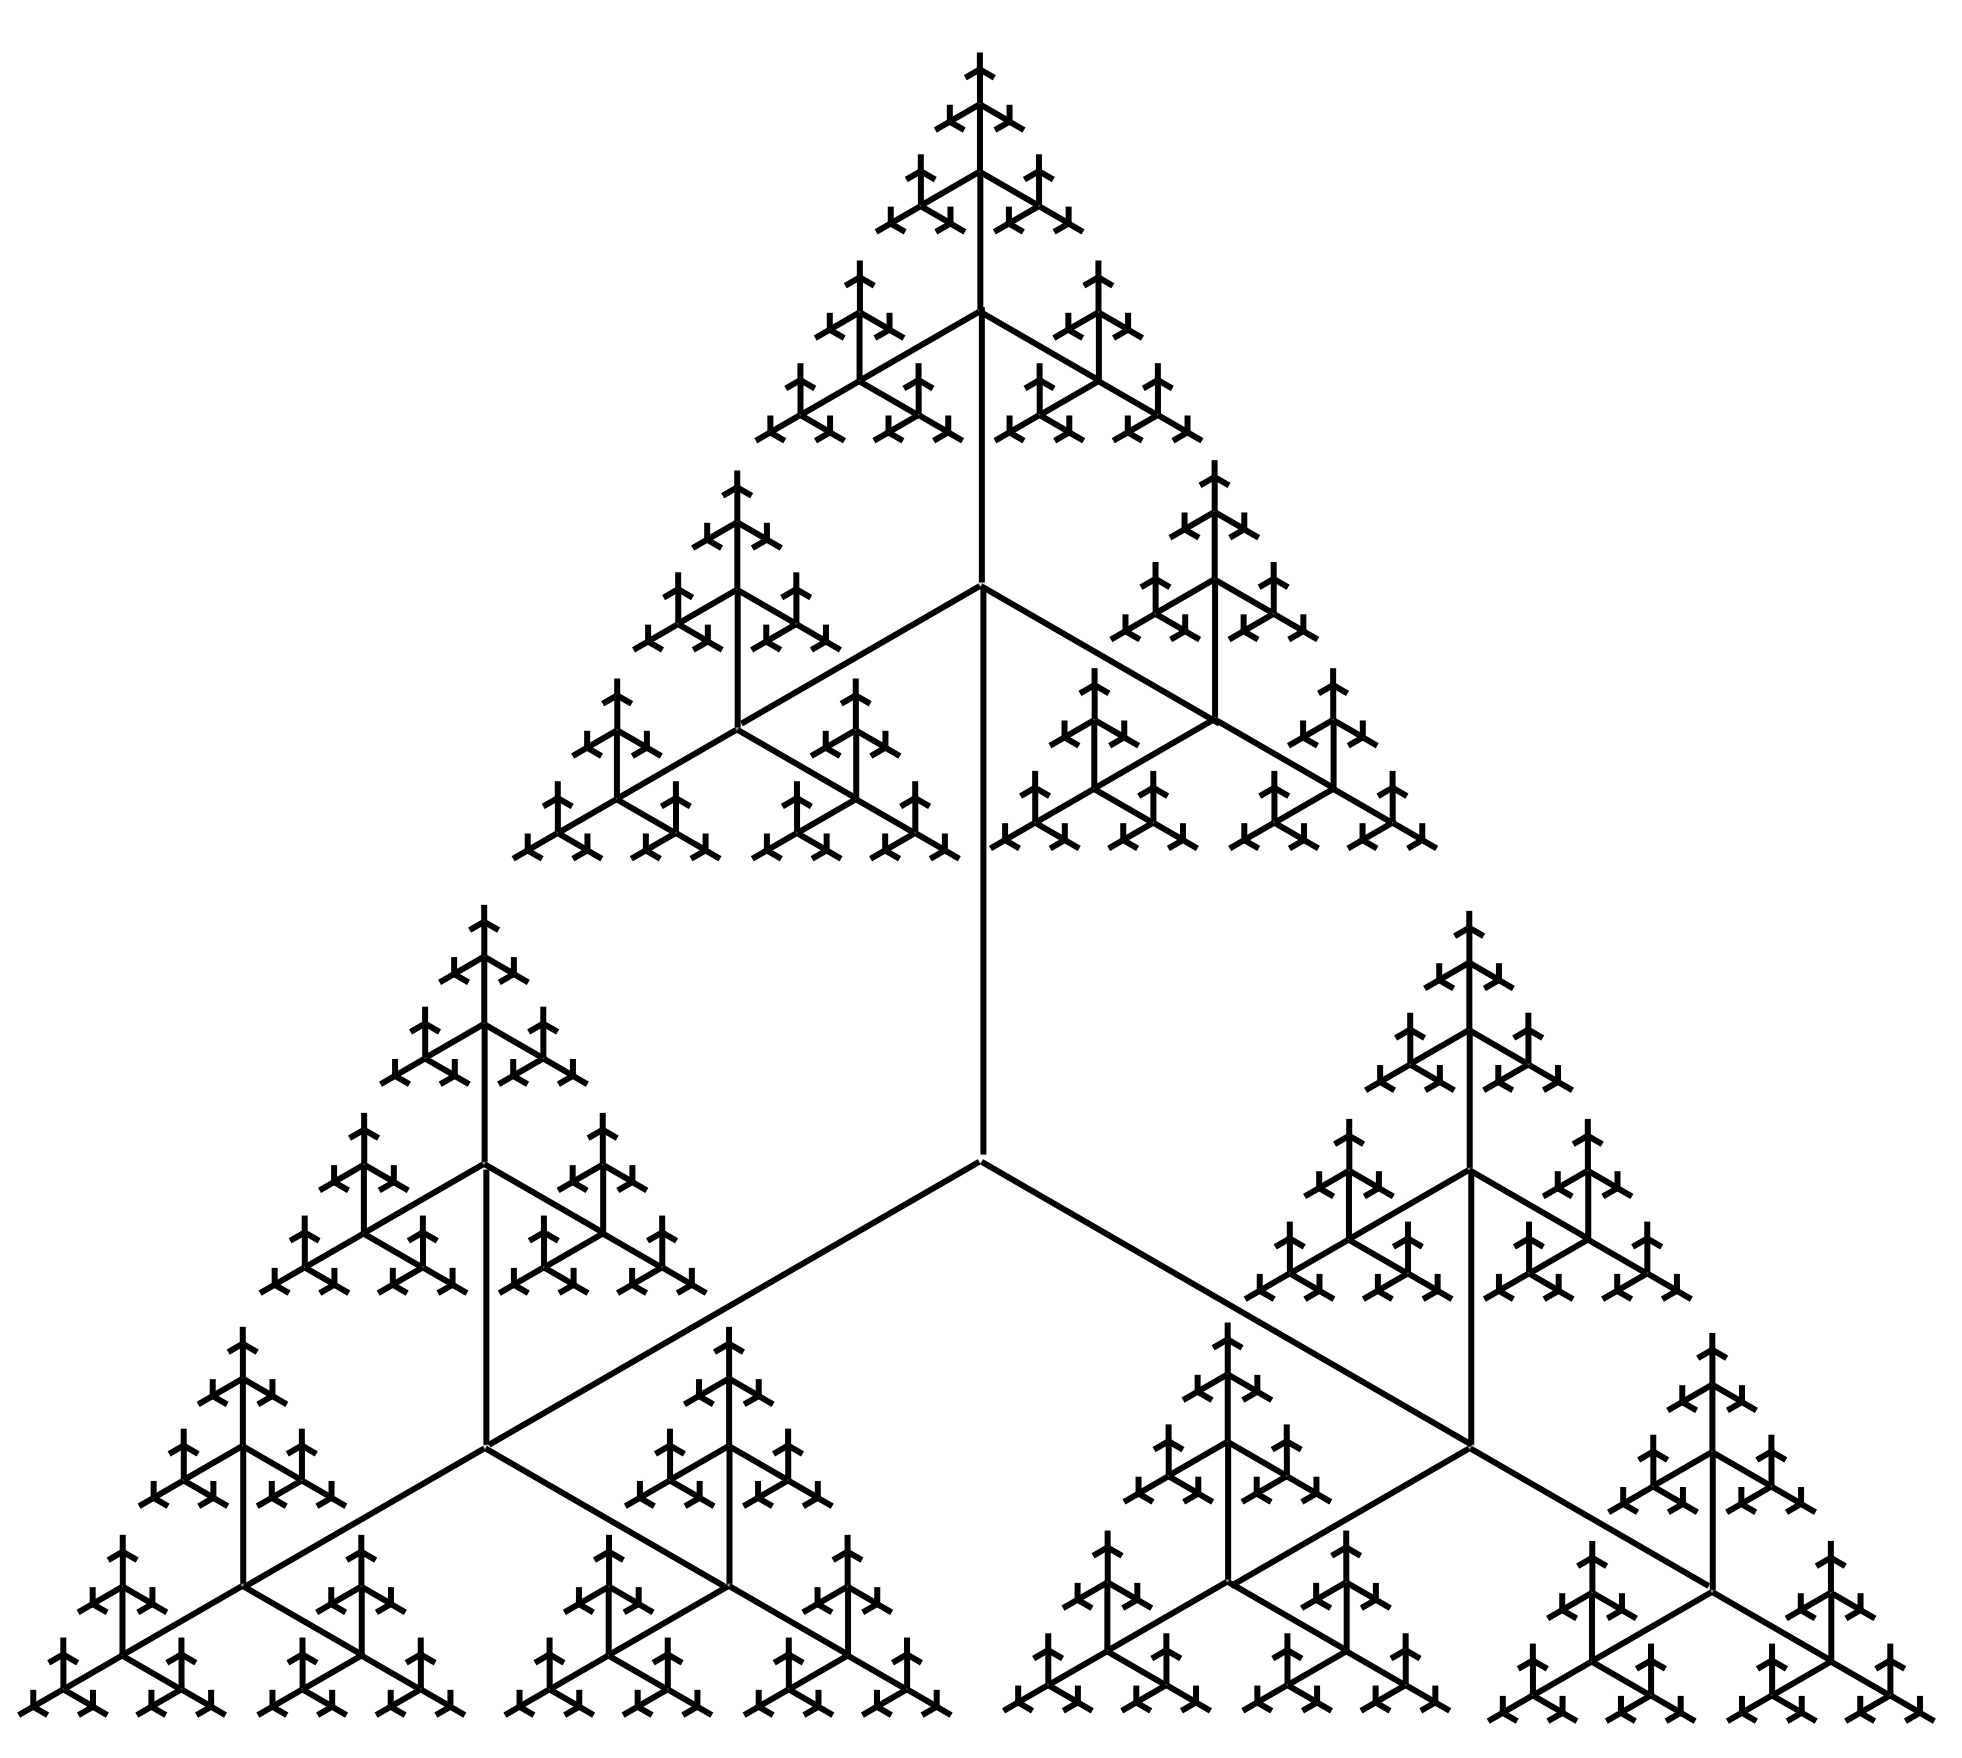
\includegraphics[scale=.1]{3_adic_Berkovich.jpg}};
	(-34,-29.5)*+{\text{{\smaller\smaller\color{blue} $\bullet$}}};
	(-35.5,-30)*+{\text{{\smaller\smaller\color{blue} $0$}}};
	(-17,-29.5)*+{\text{{\smaller\smaller\color{blue} $\bullet$}}};
	(-17,-31.5)*+{\text{{\smaller\smaller\color{blue} $3$}}};
	(-25.5,-29.5)*+{\text{{\smaller\smaller\color{blue} $\bullet$}}};
	(-25.5,-31.5)*+{\text{{\smaller\smaller\color{blue} $3^2$}}};
	(-30,-29.5)*+{\text{{\smaller\smaller\color{blue} $\bullet$}}};
	(-30,-31.5)*+{\text{{\smaller\smaller\color{blue} $3^3$}}};
	(34,-29.75)*+{\text{{\smaller\smaller\color{blue} $\bullet$}}};
	(49,-30)*+{\text{{\smaller\smaller\color{blue} $1+3+3^2+3^3+\cdots$}}};
	(.7,-29.45)*+{\text{{\smaller\smaller\color{blue} $\bullet$}}};
	(.7,-31.75)*+{\text{{\smaller\smaller\color{blue} $1$}}};
	(17.75,-29.8)*+{\text{{\smaller\smaller\color{blue} $\bullet$}}};
	(17.75,-31.95)*+{\text{{\smaller\smaller\color{blue} $1+3$}}};
	(17.25,-.8)*+{\text{{\smaller\smaller\color{blue} $\bullet$}}};
	(36.25,-.5)*+{\text{{\smaller\smaller\color{blue} $1+2\!\cdot\!3+2\!\cdot\!3^2+2\!\cdot\!3^3+\cdots$}}};
	(-16.8,.6)*+{\text{{\smaller\smaller\color{blue} $\bullet$}}};
	(-18.5,.75)*+{\text{{\smaller\smaller\color{blue} $2$}}};
	(0,29.5)*+{\text{{\smaller\smaller\color{blue} $\bullet$}}};
	(17,32)*+{\text{{\smaller\smaller\color{blue} $2+2\!\cdot\!3+2\!\cdot\!3^2+2\!\cdot\!3^3+\cdots$}}};
	(-8.2,.6)*+{\text{{\smaller\smaller\color{blue} $\bullet$}}};
	(-7.5,-1.5)*+{\text{{\smaller\smaller\color{blue} $2+3^2$}}};
	(.85,1)*+{\text{{\smaller\smaller\color{blue} $\bullet$}}};
	(4.5,-1.2)*+{\text{{\smaller\smaller\color{blue} $2+3$}}};
	(-8.1,15.3)*+{\text{{\smaller\smaller\color{blue} $\bullet$}}};
	(-13.5,16.3)*+{\text{{\smaller\smaller\color{blue} $2+2\!\cdot\!3$}}};
	(26,5.5)*+{
	\begin{tikzpicture}
	\draw[black, thick, dashed, ->] (0,0) -- (3 * 1.73205080757,3.1);
	\end{tikzpicture}
	};
	(34, 13)*+{\rotatebox{31}{{\smaller to the rest of $\QQ_3$...}}};
	(-35,20.5)*+{
	\begin{tikzpicture}
	\draw[gray, thick, ->] (0,0) -- (.5 * 1.73205080757, -.5);
	\draw[gray, thick, ->] (0,0) -- (-.5 * 1.73205080757, -.5);
	\draw[gray, thick, ->] (0,0) -- (0, 1);
	\node[gray] at (-.6 * 1.73205080757, -.6) {\scalebox{.8}{$0$}};
	\node[gray] at (.6 * 1.73205080757, -.6) {\scalebox{.8}{$1$}};
	\node[gray] at (0, 1.3) {\scalebox{.8}{$2$}};
	\end{tikzpicture}
	};
	\end{xy}
	$$
	\vskip -.3cm
	\caption{{\bf The 3-adic unit Berkovich disk $\pmb{\mathscr{M}\big(\QQ_3\langle s\rangle\big)}$.} One way to understand this figure is as the decision tree for the (countably infinite) algorithm for writing down an arbitrary $3$-adic integer. One starts at the center of the figure. Each move down a successively shorter edge of the tree determines one more $3$-adic digit, according to the rule given by the key at top left.}
	\end{figure}
\ 
{\color{red} [...]}
\end{subsection}

\begin{subsection}{One approach to {\em p}-adic signals.}
It is well known that $\QQ_2$ is homeomorphic to the standard ``middle thirds'' Cantor set inside the real interval $[0,1]$, and that $\QQ_p$ is homeomorphic to an ``alternating $(2n-1)^\text{ths}$'' Cantor-like set inside the real interval $[0,1]$.
	\begin{figure}[ht]
	$$
	\text{Step}\ 0:
	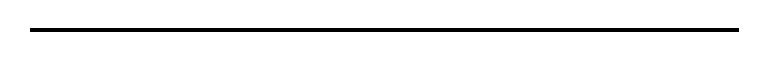
\begin{tikzpicture}
	\draw[black, ultra thick] (0,0) -- (9,0);
	\end{tikzpicture}
	$$
	$$
	\text{Step}\ 1:
	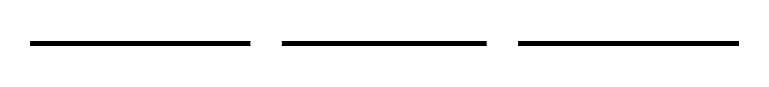
\begin{tikzpicture}
	\draw[black, ultra thick] (0,0) -- (9,0);
	%
	\fill[white] (3,0) circle (.2);
	\fill[white] (6,0) circle (.2);
	\end{tikzpicture}
	$$
	$$
	\text{Step}\ 2:
	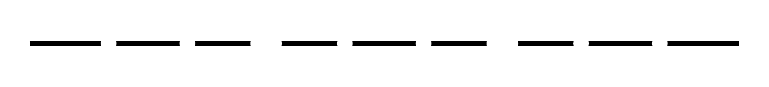
\begin{tikzpicture}
	\draw[black, ultra thick] (0,0) -- (9,0);
	%
	\fill[white] (3,0) circle (.2);
	\fill[white] (6,0) circle (.2);
	%
	\fill[white] (1,0) circle (.1);
	\fill[white] (2,0) circle (.1);
	\fill[white] (4,0) circle (.1);
	\fill[white] (5,0) circle (.1);
	\fill[white] (7,0) circle (.1);
	\fill[white] (8,0) circle (.1);
	\end{tikzpicture}
	$$
	$$
	\ \ \ \ \ \ \vdots  \ \ \ \ :
	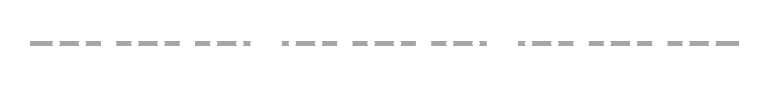
\begin{tikzpicture}
	\draw[black!35, ultra thick] (0,0) -- (9,0);
	%
	\fill[white] (3,0) circle (.2);
	\fill[white] (6,0) circle (.2);
	%
	\fill[white] (1,0) circle (.1);
	\fill[white] (2,0) circle (.1);
	\fill[white] (4,0) circle (.1);
	\fill[white] (5,0) circle (.1);
	\fill[white] (7,0) circle (.1);
	\fill[white] (8,0) circle (.1);
	%
	\fill[white] (1/3,0) circle (.05);
	\fill[white] (2/3,0) circle (.05);
	\fill[white] (1+1/3,0) circle (.05);
	\fill[white] (1+2/3,0) circle (.05);
	\fill[white] (2+1/3,0) circle (.05);
	\fill[white] (2+2/3,0) circle (.05);
	\fill[white] (3+1/3,0) circle (.05);
	\fill[white] (3+2/3,0) circle (.05);
	\fill[white] (4+1/3,0) circle (.05);
	\fill[white] (4+2/3,0) circle (.05);
	\fill[white] (5+1/3,0) circle (.05);
	\fill[white] (5+2/3,0) circle (.05);
	\fill[white] (6+1/3,0) circle (.05);
	\fill[white] (6+2/3,0) circle (.05);
	\fill[white] (7+1/3,0) circle (.05);
	\fill[white] (7+2/3,0) circle (.05);
	\fill[white] (8+1/3,0) circle (.05);
	\fill[white] (8+2/3,0) circle (.05); y
	\end{tikzpicture}
	$$
	\caption{{\bf Cantor-like, ``alternating fifths'' realization of $\pmb{\QQ_3}$.} {\color{red} [...]}} 
	\end{figure}

{\color{red} [...]}
	\begin{figure}[ht]
	$$
	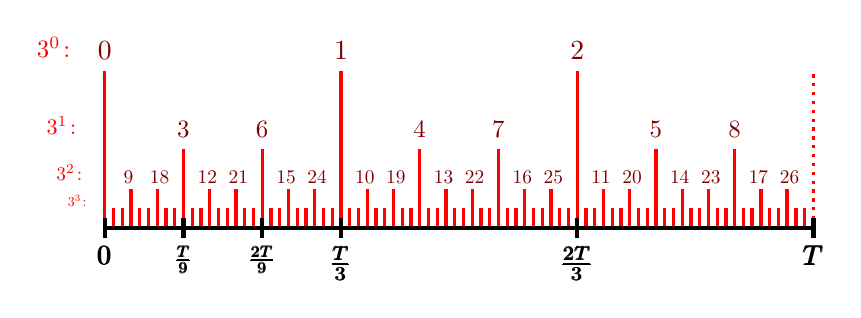
\begin{tikzpicture}
	\draw[red, very thick] (0,0) -- (0,2);
	\draw[red, very thick] (3,0) -- (3,2);
	\draw[red, very thick] (6,0) -- (6,2);
	\draw[red, very thick, dotted] (9,0) -- (9,2);
	%
	\draw[red, very thick] (1,0) -- (1,1);
	\draw[red, very thick] (2,0) -- (2,1);
	\draw[red, very thick] (4,0) -- (4,1);
	\draw[red, very thick] (5,0) -- (5,1);
	\draw[red, very thick] (7,0) -- (7,1);
	\draw[red, very thick] (8,0) -- (8,1);
	%
	\draw[red, very thick] (1/3,0) -- (1/3,.5);
	\draw[red, very thick] (2/3,0) -- (2/3,.5);
	\draw[red, very thick] (1+1/3,0) -- (1+1/3,.5);
	\draw[red, very thick] (1+2/3,0) -- (1+2/3,.5);
	\draw[red, very thick] (2+1/3,0) -- (2+1/3,.5);
	\draw[red, very thick] (2+2/3,0) -- (2+2/3,.5);
	\draw[red, very thick] (3+1/3,0) -- (3+1/3,.5);
	\draw[red, very thick] (3+2/3,0) -- (3+2/3,.5);
	\draw[red, very thick] (4+1/3,0) -- (4+1/3,.5);
	\draw[red, very thick] (4+2/3,0) -- (4+2/3,.5);
	\draw[red, very thick] (5+1/3,0) -- (5+1/3,.5);
	\draw[red, very thick] (5+2/3,0) -- (5+2/3,.5);
	\draw[red, very thick] (6+1/3,0) -- (6+1/3,.5);
	\draw[red, very thick] (6+2/3,0) -- (6+2/3,.5);
	\draw[red, very thick] (7+1/3,0) -- (7+1/3,.5);
	\draw[red, very thick] (7+2/3,0) -- (7+2/3,.5);
	\draw[red, very thick] (8+1/3,0) -- (8+1/3,.5);
	\draw[red, very thick] (8+2/3,0) -- (8+2/3,.5);
	%
	\draw[red, very thick] (1/9,0) -- (1/9,.25);
	\draw[red, very thick] (2/9,0) -- (2/9,.25);
	\draw[red, very thick] (1/3+1/9,0) -- (1/3+1/9,.25);
	\draw[red, very thick] (1/3+2/9,0) -- (1/3+2/9,.25);
	\draw[red, very thick] (2/3+1/9,0) -- (2/3+1/9,.25);
	\draw[red, very thick] (2/3+2/9,0) -- (2/3+2/9,.25);
	\draw[red, very thick] (3/3+1/9,0) -- (3/3+1/9,.25);
	\draw[red, very thick] (3/3+2/9,0) -- (3/3+2/9,.25);
	\draw[red, very thick] (4/3+1/9,0) -- (4/3+1/9,.25);
	\draw[red, very thick] (4/3+2/9,0) -- (4/3+2/9,.25);
	\draw[red, very thick] (5/3+1/9,0) -- (5/3+1/9,.25);
	\draw[red, very thick] (5/3+2/9,0) -- (5/3+2/9,.25);
	\draw[red, very thick] (6/3+1/9,0) -- (6/3+1/9,.25);
	\draw[red, very thick] (6/3+2/9,0) -- (6/3+2/9,.25);
	\draw[red, very thick] (7/3+1/9,0) -- (7/3+1/9,.25);
	\draw[red, very thick] (7/3+2/9,0) -- (7/3+2/9,.25);
	\draw[red, very thick] (8/3+1/9,0) -- (8/3+1/9,.25);
	\draw[red, very thick] (8/3+2/9,0) -- (8/3+2/9,.25);
	\draw[red, very thick] (9/3+1/9,0) -- (9/3+1/9,.25);
	\draw[red, very thick] (9/3+2/9,0) -- (9/3+2/9,.25);
	\draw[red, very thick] (10/3+1/9,0) -- (10/3+1/9,.25);
	\draw[red, very thick] (10/3+2/9,0) -- (10/3+2/9,.25);
	\draw[red, very thick] (11/3+1/9,0) -- (11/3+1/9,.25);
	\draw[red, very thick] (11/3+2/9,0) -- (11/3+2/9,.25);
	\draw[red, very thick] (12/3+1/9,0) -- (12/3+1/9,.25);
	\draw[red, very thick] (12/3+2/9,0) -- (12/3+2/9,.25);
	\draw[red, very thick] (13/3+1/9,0) -- (13/3+1/9,.25);
	\draw[red, very thick] (13/3+2/9,0) -- (13/3+2/9,.25);
	\draw[red, very thick] (14/3+1/9,0) -- (14/3+1/9,.25);
	\draw[red, very thick] (14/3+2/9,0) -- (14/3+2/9,.25);
	\draw[red, very thick] (15/3+1/9,0) -- (15/3+1/9,.25);
	\draw[red, very thick] (15/3+2/9,0) -- (15/3+2/9,.25);
	\draw[red, very thick] (16/3+1/9,0) -- (16/3+1/9,.25);
	\draw[red, very thick] (16/3+2/9,0) -- (16/3+2/9,.25);
	\draw[red, very thick] (17/3+1/9,0) -- (17/3+1/9,.25);
	\draw[red, very thick] (17/3+2/9,0) -- (17/3+2/9,.25);
	\draw[red, very thick] (18/3+1/9,0) -- (18/3+1/9,.25);
	\draw[red, very thick] (18/3+2/9,0) -- (18/3+2/9,.25);
	\draw[red, very thick] (19/3+1/9,0) -- (19/3+1/9,.25);
	\draw[red, very thick] (19/3+2/9,0) -- (19/3+2/9,.25);
	\draw[red, very thick] (20/3+1/9,0) -- (20/3+1/9,.25);
	\draw[red, very thick] (20/3+2/9,0) -- (20/3+2/9,.25);
	\draw[red, very thick] (21/3+1/9,0) -- (21/3+1/9,.25);
	\draw[red, very thick] (21/3+2/9,0) -- (21/3+2/9,.25);
	\draw[red, very thick] (22/3+1/9,0) -- (22/3+1/9,.25);
	\draw[red, very thick] (22/3+2/9,0) -- (22/3+2/9,.25);
	\draw[red, very thick] (23/3+1/9,0) -- (23/3+1/9,.25);
	\draw[red, very thick] (23/3+2/9,0) -- (23/3+2/9,.25);
	\draw[red, very thick] (24/3+1/9,0) -- (24/3+1/9,.25);
	\draw[red, very thick] (24/3+2/9,0) -- (24/3+2/9,.25);
	\draw[red, very thick] (25/3+1/9,0) -- (25/3+1/9,.25);
	\draw[red, very thick] (25/3+2/9,0) -- (25/3+2/9,.25);
	\draw[red, very thick] (26/3+1/9,0) -- (26/3+1/9,.25);
	\draw[red, very thick] (26/3+2/9,0) -- (26/3+2/9,.25);
	%
	\draw[black, ultra thick] (0,0) -- (9,0);
	%
	\node[red] at (-.65,2.3) {\scalebox{.9}{$3^0\!:$}};
	\node[red] at (-.55,1.3) {\scalebox{.8}{$3^1\!:$}};
	\node[red] at (-.45,.7) {\scalebox{.7}{$3^2\!:$}};
	\node[red] at (-.35,.35) {\scalebox{.5}{$3^3\!:$}};
	%
	\node[red!50!black!100] at (0,2.25) {\scalebox{1}{$0$}};
	\node[red!50!black!100] at (3,2.25) {\scalebox{1}{$1$}};
	\node[red!50!black!100] at (6,2.25) {\scalebox{1}{$2$}};
	%
	\node[red!50!black!100] at (1,1.25) {\scalebox{.9}{$3$}};
	\node[red!50!black!100] at (2,1.25) {\scalebox{.9}{$6$}};
	\node[red!50!black!100] at (4,1.25) {\scalebox{.9}{$4$}};
	\node[red!50!black!100] at (5,1.25) {\scalebox{.9}{$7$}};
	\node[red!50!black!100] at (7,1.25) {\scalebox{.9}{$5$}};
	\node[red!50!black!100] at (8,1.25) {\scalebox{.9}{$8$}};
	%
	\node[red!50!black!100] at (1/3,.65) {\scalebox{.7}{$9\ $}};
	\node[red!50!black!100] at (2/3,.65) {\scalebox{.7}{$\ 18$}};
	\node[red!50!black!100] at (1+1/3,.65) {\scalebox{.7}{$12\ $}};
	\node[red!50!black!100] at (1+2/3,.65) {\scalebox{.7}{$\ 21$}};
	\node[red!50!black!100] at (2+1/3,.65) {\scalebox{.7}{$15\ $}};
	\node[red!50!black!100] at (2+2/3,.65) {\scalebox{.7}{$\ 24$}};
	\node[red!50!black!100] at (3+1/3,.65) {\scalebox{.7}{$10\ $}};
	\node[red!50!black!100] at (3+2/3,.65) {\scalebox{.7}{$\ 19$}};
	\node[red!50!black!100] at (4+1/3,.65) {\scalebox{.7}{$13\ $}};
	\node[red!50!black!100] at (4+2/3,.65) {\scalebox{.7}{$\ 22$}};
	\node[red!50!black!100] at (5+1/3,.65) {\scalebox{.7}{$16\ $}};
	\node[red!50!black!100] at (5+2/3,.65) {\scalebox{.7}{$\ 25$}};
	\node[red!50!black!100] at (6+1/3,.65) {\scalebox{.7}{$11\ $}};
	\node[red!50!black!100] at (6+2/3,.65) {\scalebox{.7}{$\ 20$}};
	\node[red!50!black!100] at (7+1/3,.65) {\scalebox{.7}{$14\ $}};
	\node[red!50!black!100] at (7+2/3,.65) {\scalebox{.7}{$\ 23$}};
	\node[red!50!black!100] at (8+1/3,.65) {\scalebox{.7}{$17\ $}};
	\node[red!50!black!100] at (8+2/3,.65) {\scalebox{.7}{$\ 26$}};
	%
	\draw[black, ultra thick] (0,.125) -- (0,-.125);
	\draw[black, ultra thick] (1,.125) -- (1,-.125);
	\draw[black, ultra thick] (2,.125) -- (2,-.125);
	\draw[black, ultra thick] (3,.125) -- (3,-.125);
	\draw[black, ultra thick] (6,.125) -- (6,-.125);
	\draw[black, ultra thick] (9,.125) -- (9,-.125);
	%
	\node[black] at (0,-.35) {\scalebox{1}{$\pmb{0}$}};
	\node[black] at (1,-.4) {\scalebox{.8}{$\pmb{\frac{T}{9}}$}};
	\node[black] at (2,-.4) {\scalebox{.8}{$\pmb{\frac{2T}{9}}$}};
	\node[black] at (3,-.45) {\scalebox{1}{$\pmb{\frac{T}{3}}$}};
	\node[black] at (6,-.45) {\scalebox{1}{$\pmb{\frac{2T}{3}}$}};
	\node[black] at (9,-.35) {\scalebox{1}{$\pmb{T}$}};
	\end{tikzpicture}
	$$
	\caption{{\bf Proposed ``{\em p}-adic'' signal approximation in the case $\pmb{p=3}$.}\ {\color{red} [$\frac{T}{p^n}$-sample per second signal approximation... Explain that the specific indexing of the samples indicated in this figure is critical to the harmonic/tonal movement...]} {\color{red} [Explain how this can viewed as an actual signal over $\QQ_{p}$ with its correct topology, with a bit of signal inertia...]}}
	\label{figure: p-adic signal proposal}
	\end{figure}
	
{\color{red} [Makes Fourier transformation integrals volumetrically correct. Does {\em not} preserve addition. ...What are the musical consequences of this?...]}

\begin{algorithm}
\caption{$p$-Adic coordinates, at resolution-$p^m$, for non-negative real numbers}\label{algorithm: weak p-adic coordinate}
\KwData{positive prime $p\in\ZZ_{>0}$, non-negative real $t\in\RR_{\ge0}$, positive integer $m\in\ZZ_{>0}$}
\KwResult{$p$-adic number $a\in\QQ_{p}$ and non-negative real error $\varepsilon\in\RR_{\ge0}$ such that $t=a+\varepsilon$}
$\varepsilon \gets$ {\bf copy of real number} $t$ \label{line: define r} \tcp*[r]{running error, to modify over course of algorithm}
$n \gets$ {\bf integer} $0$\; \label{line: define n}
\While{$p^{n} \le \varepsilon$
}{
    $n \gets n+1$ \label{line: increase n by 1}  \tcp*[r]{\ref{line: define n}-\ref{line: increase n by 1} end with $n\in\ZZ_{\ge 0}$ such that  $p^{n-1}\le \varepsilon<p^{n}$}
}
$a \gets$ {\bf {\em p}-adic number} $0$
\; \label{line: define p-adic to update}
\For{$i\gets n-1$ \KwTo $-m$ \KwBy $-1$
}{
$a_{-i}=\lfloor\tfrac{\varepsilon}{p^i}\rfloor$ \tcp*[r]{$a_{-i}\in\ZZ$ satisfies $0\le a_{-i}<p$ and $a_{-i}p^n\le \varepsilon<(a_{-i}+1)p^{n}$}
%\While{$(a_{-i}+1)\cdot p^i\le r$}{
%$a_{-i}\gets a_{-i}+1$ \;
%}
$\varepsilon\gets$ {\bf real number} $\varepsilon-a_{-i}p^{i}$ \;
{$a \gets$ {\bf {\em p}-adic number} $a+a_{-i}p^{-i}$} \tcp*[r]{\ref{line: define p-adic to update}-\ref{line: p-adic update} end with $p$-adic number $a=\sum_{j=-m}^{n-1}a_jp^j$}
\label{line: p-adic update}}
{\bf return} $a$,\ \ $\varepsilon$,\ \  $n-1$ \tcp*[r]{Interpreting $a$ as $\in\QQ$, we have $t=\varepsilon+a$, with $0\le \varepsilon<\tfrac{1}{p^{m}}$.} 
\end{algorithm}

Taking the first output $a$ of Algorithm \ref{algorithm: weak p-adic coordinate} gives us with a map
	%\begin{equation}\label{equation: weak inverse pre-embed}
	$
	\RR_{\ge0}\longrightarrow\tfrac{1}{p^m}\ZZ,
	$
	%\end{equation}
which we can interpret as a map into $\QQ_{p}$ via the natural inclusions
	$$
	\tfrac{1}{p^m}\ZZ
	\ \subset\ 
	\ZZ\big[\tfrac{1}{p}\big]
	\ \subset\ 
	\QQ_{p}.
	$$
The resulting map
	\begin{equation}\label{equation: weak inverse from algorithm}
	\text{adic}_{p^m}:\RR_{\ge0}\longrightarrow\QQ_p
	\end{equation}
provides a ``resolution-$p^{m}$ weak inverse'' to the map
	\begin{equation}\label{equation: p-adic to real}
	\text{real}:\QQ_{p}\longrightarrow\RR_{\ge0}
	\end{equation}
that S.V. Kozyrev denotes ``$\rho$'' in \cite[p. 7, Equation (12)]{Kozyrev}. This map in Equation \eqref{equation: p-adic to real} is given by
	$$
	\text{real}\big(a_{-n}\tfrac{1}{p^{n}}+\cdots+a_{-1}\tfrac{1}{p}+a_0+a_1 p+\cdots\big)
	\ =\ 
	a_{-n}p^{n-1}+\cdots+a_{-1}+a_0\tfrac{1}{p}+a_1\tfrac{1}{p^{2}}+\cdots
	$$
{\color{red} [Need to make indexing here match indexing in Algorithm \ref{algorithm: weak p-adic coordinate}]}
Kozyrev points out that this map $\text{real}$ induces a unitary map between the associated $L^2$ spaces, and takes the Haar wavelet to our character $\chi_{\text{{\smaller\smaller\smaller $\tfrac{1}{p}$}}}$ on the dyadics, i.e., in the special case $p=2$:

\begin{lemma}\label{lemma: Kozyrev}
\normalfont
\cite[Lemmas 5 \& 6]{Kozyrev}
The map $\text{real}:\QQ_{p}\longrightarrow\RR_{\ge0}$ induces a unitary embedding
	$$
	\text{real}^\ast:L^2(\RR_{\ge0},\CC)\mono L^2(\QQ_{p},\CC).
	$$
In the special case that $p=2$, this unitary embedding
that takes the Haar wavelet $$\psi_{\text{Haar}}:=\mathbbm{1}_{[0,\text{{\smaller\smaller\smaller $\tfrac{1}{2}$}}]}-\mathbbm{1}_{[\text{{\smaller\smaller\smaller $\tfrac{1}{2}$}},1]}$$ to the character $\chi_{\text{{\smaller\smaller\smaller $\tfrac{1}{2}$}}}$:

\hfill \ \ $
	\text{real}^\ast\psi_{\text{Haar}}
	\ =\ 
	\chi_{\text{{\smaller\smaller\smaller $\tfrac{1}{2}$}}}.
 	$
\hfill $\qed$
\end{lemma}

More generally, if we let $\zeta_p$ denote the $p^\text{th}$ primitive root of unity $\zeta=e^{i2\pi\text{{\smaller\smaller\smaller$\tfrac{1}{p}$}}}$, then we have
	$$
	\text{real}^\ast\Big(\sum_{n=0}^{p-1}\zeta^{n}_p\cdot\mathbbm{1}_{[\text{{\smaller\smaller\smaller $\tfrac{n}{p}$}},\text{{\smaller\smaller\smaller $\tfrac{n+1}{p}$}}]}\Big)
	\ =\ 
	\chi_{\text{{\smaller\smaller\smaller $\tfrac{1}{p}$}}}
	$$
{\color{red} [Is it true that
	\begin{equation}\label{equation: general roots of unity wavelet}
	\text{real}^\ast\Big(\sum_{n=0}^{p^{k}-1}\zeta^{n}_{p^k}\cdot\mathbbm{1}_{[\text{{\smaller\smaller\smaller $\tfrac{n}{p^k}$}},\text{{\smaller\smaller\smaller $\tfrac{n+1}{p^k}$}}]}\Big)
	\ \overset{?}{=}\ 
	\chi_{\text{{\smaller\smaller\smaller $\tfrac{1}{p^k}$}}}
	\end{equation}
The odd way that integers get distributed across $p$-adic coordinates in $\RR_{\ge 0}$ make me suspicious that this is too much to ask for...]}

\begin{question}
{\bf Implications of measure coincidence?}
\normalfont
Kozyrev's Lemma \ref{lemma: Kozyrev} implies that for any function $f\in L^{2}(\QQ_{p}, \CC)$ that can be obtained as a pullback
	$$
	f\ =\ \text{real}^\ast g
	\ \ \ \text{for some}\ g\in L^2(\RR_{\ge0},\CC),
	$$
and for any compact region $U\subset \QQ_{p}$, we can compute the integral $\int_{U}f\ d\mu_p$ over $\RR_{\ge0}$ as
	$$
	\int_{U}f\ d\mu_p
	\ =\ 
	\int_{U}\text{real}^{\ast}\!g\  d\mu_{p}
	\ =\ 
	\int_{\text{real}(U)}g\ d\mu_{\infty}.
	$$
For example, if $f=\text{real}^\ast g$, then
	$$
	\int_{\QQ_{p}}f\cdot\chi_{\text{{\smaller\smaller\smaller $\tfrac{1}{p}$}}}\ d\mu_p
	\ =\ 
	\sum_{n=0}^{p-1}\ \zeta^{n}_p\cdot\int^{\text{{\smaller\smaller\smaller $\tfrac{n+1}{p}$}}}_{\!\text{{\smaller\smaller\smaller $\tfrac{n}{p}$}}}
	\!\!\!\!g\ d\mu_\infty
	$$
Does this have sonic/musical implications? What sorts of $p$-adic ``things'' become audible under the unitary embedding $\text{real}^\ast:L^2(\RR_{\ge0},\CC)\mono L^2(\QQ_{p},\CC)$? For instance, does the correct version of Equation \eqref{equation: general roots of unity wavelet} imply that $p$-adic spectral analysis becomes a sort of strange wavelet analysis on $\RR_{\ge0}$? What sorts of sonically/musically ``things'' are the {\em generalized} Haar signals good at keeping track of?
\end{question}

\begin{construction}
	\normalfont

	$$
	\begin{xy}
	(0,0)*+{\RR_{\ge0}}="0";
	(30,10)*+{\{0,\ \!\dots,\ \!p-1\}^{\NN}}="2";
	(30,-10)*+{\QQ}="3";
	(60,-10)*+{\overset{\ }{\QQ}_{\ }}="4";
	(60,10)*+{\QQ_p}="5";
	(90,10)*+{\QQ_p/\ZZ_{p}}="6";
	(90,-10)*+{\QQ/\ZZ}="8";
	(120,0)*+{\CC}="9";
	{\ar@/^10pt/_{\!\!\!\!\!\!\!\!\!\!\!\!\!\!\rotatebox{30}{{\smaller\smaller $\text{adic}_{p^m}$}}} "0"; "2"};
	{\ar^{\rotatebox{-90}{{\smaller\smaller $\text{rational}$}}} "2"; "3"};
	{\ar^{b\cdot(-)} "3"; "4"};
	{\ar@{^{(}->} "4"; "5"};
	{\ar_{\lambda_1} "5"; "6"};
	{\ar^{\wr} "6"; "8"};
	{\ar@/_10pt/^{\rotatebox{15}{{\smaller\smaller $e^{i2\pi\cdot(-)}$}}\!\!\!\!} "8"; "9"};
	\end{xy}
	$$
\end{construction}

\begin{algorithm}
\caption{``Real audio signal'' (up to conductor), from $p$-adic function. Implementation of Construction [...]}\label{algorithm: UMM}
\KwData{positive prime $p\in\ZZ_{>0}$, non-negative real $t\in\RR_{\ge0}$, positive integer $m\in\ZZ_{>0}$}
\KwResult{$p$-adic number $a\in\QQ_{p}$ and non-negative real error $\varepsilon\in\RR_{\ge0}$ such that $t=a+\varepsilon$}
$\varepsilon \gets$ {\bf copy of real number} $t$ \label{line: define r} \tcp*[r]{running error, to modify over course of algorithm}
$n \gets$ {\bf integer} $0$\; \label{line: define n}
\While{$p^{n} \le \varepsilon$
}{
    $n \gets n+1$ \label{line: increase n by 1}  \tcp*[r]{\ref{line: define n}-\ref{line: increase n by 1} end with $n\in\ZZ_{\ge 0}$ such that  $p^{n-1}\le \varepsilon<p^{n}$}
}
{\bf return} $a$,\ \ $\varepsilon$,\ \  $n-1$ \tcp*[r]{Interpreting $a$ as $\in\QQ$, we have $t=\varepsilon+a$, with $0\le \varepsilon<\tfrac{1}{p^{m}}$.} 
\end{algorithm}


\begin{proposal}\label{proposal: p-adic chords}
{\bf Chords as sums of ``pure oscillators.''}
\normalfont

{\color{red} [Problem: The graphs of these oscillators are {\em really} dense... Not sure there's anything sonically interesting there...]}

	$$
	\includegraphics[scale=.33]{001.jpg}
	$$
{\color{red} [...]}
	$$
	\includegraphics[scale=.33]{002.jpg}
	$$
\end{proposal}

\begin{proposal}\label{proposal: smooth-to-p-adic}
{\bf Tones as {\em p}-adic transformations of continuous signals.}
\normalfont
	\begin{figure}[ht]
	$$
	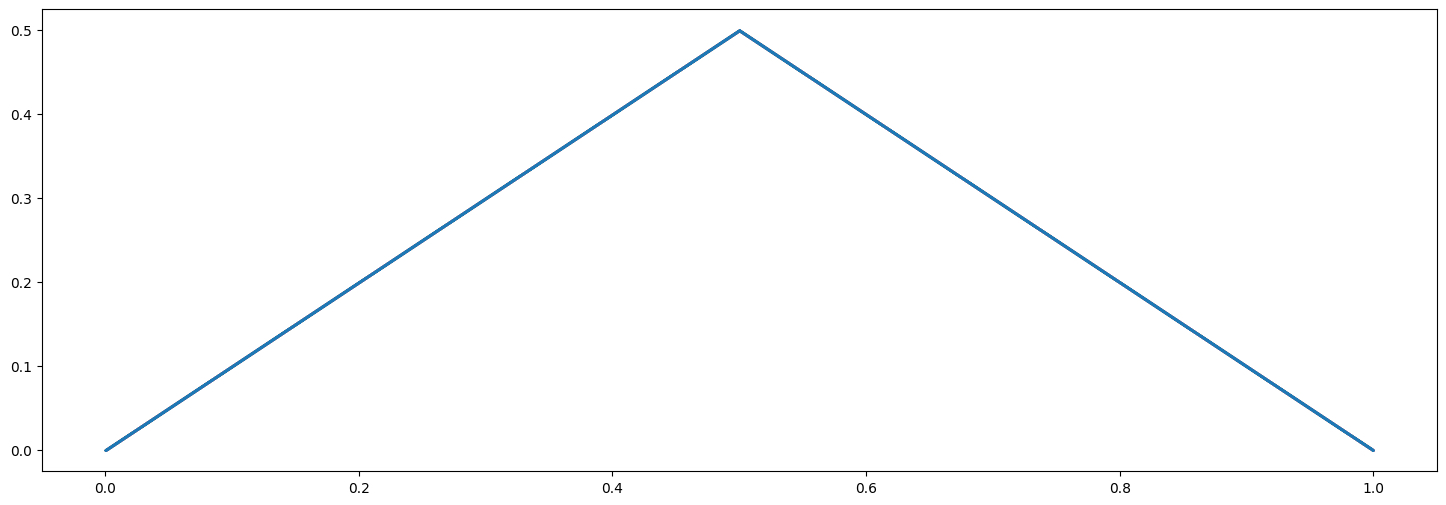
\includegraphics[scale=.3]{3-adic_triangle.jpg}
	$$
	$$
	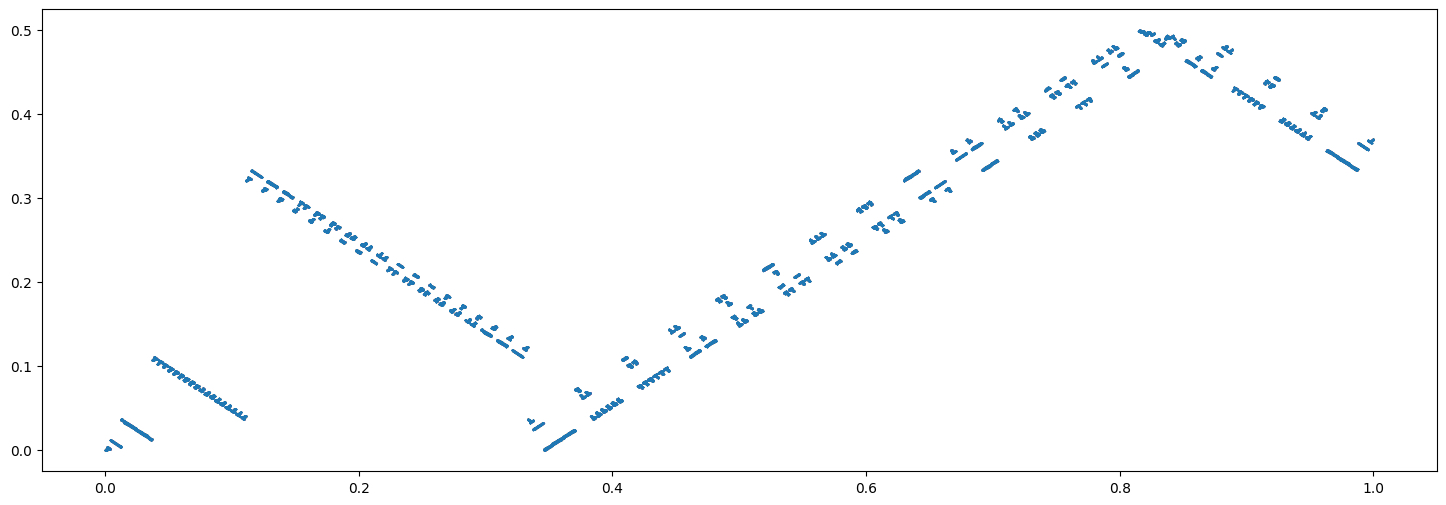
\includegraphics[scale=.3]{3-adic.jpg}
	$$
	\vskip -.3cm
	\caption{{\bf Triangle wave $\pmb{f(s)=\tfrac{1}{2}\!-\!\big|t(s)\!-\!\tfrac{1}{2}\big|}$ under 3-adic frequency transform $\pmb{\!f(s)\mapsto\!f(26\ \!s)}$.} {\color{red} [...]} One can see in this image how $p$-adic multiplication acts by ``fractal permutations'' tied to the arithmetic structure of the ring $\QQ_{p}$. The $3$-adic presentation the factor $26$ is $26=2+2\!\cdot\!3+2\!\cdot\!3^2$.}
	\end{figure}
	
{\color{red} [...]}


	\begin{figure}[ht]
	$$
	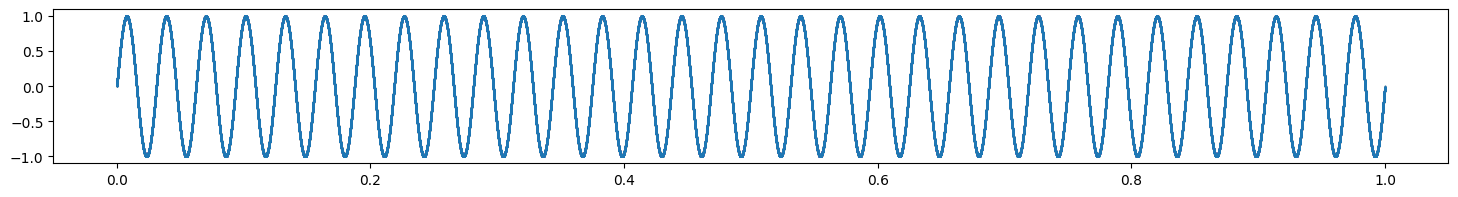
\includegraphics[scale=.420]{30-adic.png}
	$$
	$$
	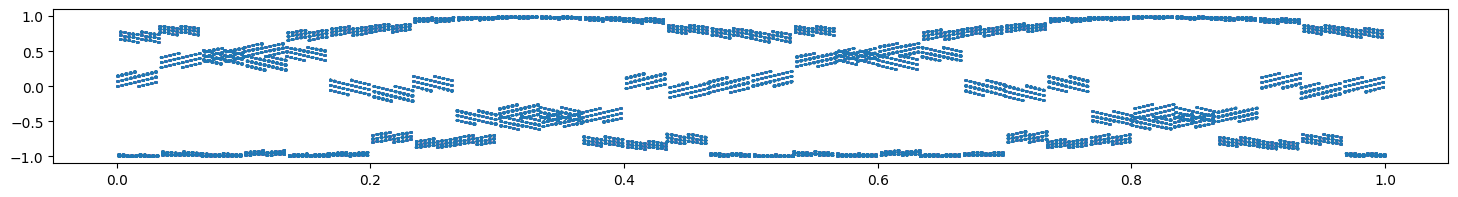
\includegraphics[scale=.420]{30-adic_by_20.png}
	$$
	$$
	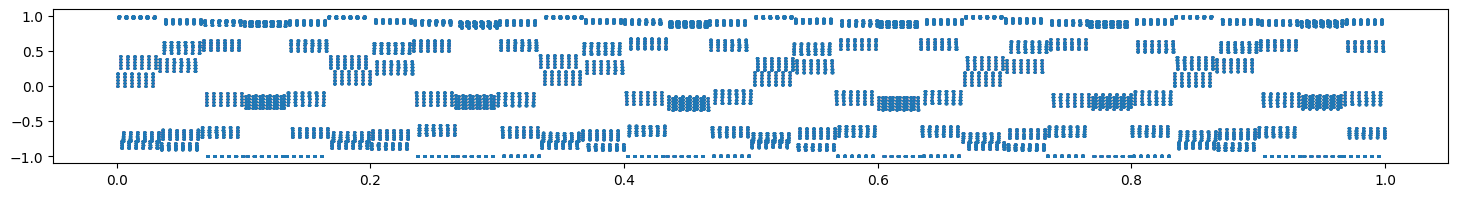
\includegraphics[scale=.420]{30-adic_by_36.png}
	$$
	$$
	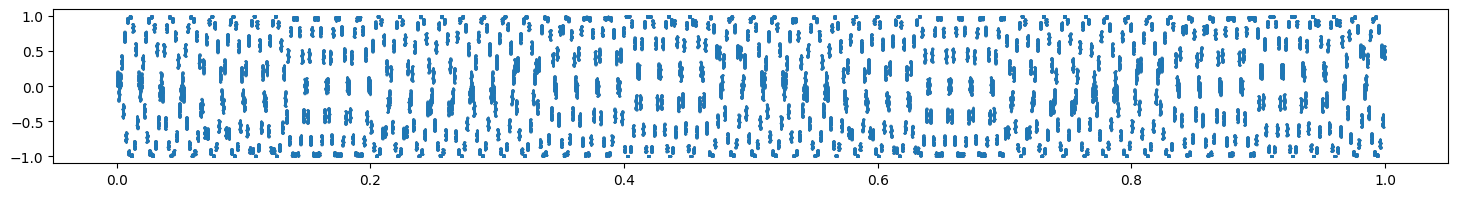
\includegraphics[scale=.420]{30-adic_by_44.png}
	$$
	\vskip -.3cm
	\caption{{\color{red} [...]} 30-adic $f(s)=\text{sin}\big(2\pi\cdot30 t(s)\big)$ by 10 and by }
	\end{figure}

{\color{red} [Problem: How does it sound?...]}
\end{proposal}

\begin{remark}
{\bf Proposals \ref{proposal: p-adic chords} and \ref{proposal: smooth-to-p-adic} are {\em not} mutually exclusive.}
\normalfont
{\color{red} [...]}
\end{remark}

\begin{remark}
{\bf An approach to {\em p}-adic signals that doesn't quite work.}
\normalfont
Another idea I had for deploying $p$-adic signals is the following:
	\begin{enumerate}[{\bf\ \ \ \ \ \ \ $\star$}]
	\item\vskip .2cm
	{\bf Another idea for realizing {\em p}-adic signals.} Use sample audio signals $f:\RR\lra\RR$ only on the rationals $\QQ\subset\RR$. Use the canonical embedding $\QQ\mono\QQ_{p}$ to reinterpret each rational argument of $f$ as a $p$-adic, and multiply the arguments of signals by $\QQ^{\times}_p$ accordingly.
	\vskip .2cm
	\end{enumerate}
The problem is that there's a fatal circularity in this idea.
{\color{red} [...]}
\end{remark}

\end{subsection}

\vskip .3cm

\begin{subsection}{{\em p}-Adic Daubechies wavelets}
\ {\color{red} [...]}
	\begin{figure}[ht]
	$$
	\scalebox{.9}{$
	\begin{xy}
	(-80,0)*+{\!\!\!\pmb{L^2(\RR)}}="-4";
	(-60,0)*+{\ \pmb{\cdots}\ }="-3";
	(-40,0)*+{\ \pmb{V_{-1}}\ }="-2";
	(-20,0)*+{\ \pmb{V_{0}}\ }="-1";
	(0,0)*+{\ \pmb{V_1}\ }="0";
	(20,0)*+{\ \pmb{\cdots}\ }="1";
	(40,0)*+{\ \pmb{V_{j}}\ }="2";
	(60,0)*+{\ \pmb{\cdots}\ }="3";
	(80,0)*+{\ \pmb{\{0\}}\ }="4";
	%
	(-65,10)*+{\text{{\color{blue}\smaller rescaling}}};
	(-66,7)*+{\text{{\color{blue}\smaller operations:}}};
	%
	(60, -19)*+{{\color{black!30!red!100} \text{topologically exhaustive:}}};
	(60, -25)*+{{\color{black!30!red!100} \pmb{\text{cl}\big(\underset{j\in\ZZ}{\bigcup}V_{j}\big)=L^2(\RR)}}};
	(60, -34)*+{{\color{black!30!red!100} \text{separated:}}};
	(60, -40)*+{\color{black!30!red!100} \pmb{\underset{j\in\ZZ}{\bigcap}V_{j}=\{0\}}};
	%
	{\ar@/^0pt/@{_{(}->} "-3"; "-4"};
	{\ar@/_37pt/@{->>}_{\text{pr}_0} "-4"; "-1"};
	{\ar@/_57pt/@{->>}_{\text{pr}_{1}} "-4"; "0"};
	{\ar@/_97pt/@{->>}_{\text{pr}_{j}} "-4"; "2"};
	%
	{\ar@[blue]@/^22pt/@{->}^{\text{{\smaller\smaller\smaller\smaller\color{blue} $1/p$}}} "-3"; "-2"};
	{\ar@[blue]@/_14pt/@{->}^{\text{{\smaller\smaller\smaller\smaller\color{blue} $p$}}} "-2"; "-3"};
	{\ar@/^0pt/@{_{(}->} "-2"; "-3"};
	{\ar@/_5pt/@{->>}_{\text{pr}^{-2}_{-1}} "-3"; "-2"};
	%
	{\ar@[blue]@/^22pt/@{->}^{\text{{\smaller\smaller\smaller\smaller\color{blue} $1/p$}}} "-2"; "-1"};
	{\ar@[blue]@/_14pt/@{->}^{\text{{\smaller\smaller\smaller\smaller\color{blue} $p$}}} "-1"; "-2"};
	{\ar@/^0pt/@{_{(}->} "-1"; "-2"};
	{\ar@/_5pt/@{->>}_{\text{pr}^{-1}_{0}} "-2"; "-1"};
	%
	{\ar@[blue]@/^22pt/@{->}^{\text{{\smaller\smaller\smaller\smaller\color{blue} $1/p$}}} "-1"; "0"};
	{\ar@[blue]@/_14pt/@{->}^{\text{{\smaller\smaller\smaller\smaller\color{blue} $p$}}} "0"; "-1"};
	{\ar@/^0pt/@{_{(}->} "0"; "-1"};
	{\ar@/_5pt/@{->>}_{\text{pr}^{0}_{1}} "-1"; "0"};
	%
	{\ar@[blue]@/^22pt/@{->}^{\text{{\smaller\smaller\smaller\smaller\color{blue} $1/p$}}} "0"; "1"};
	{\ar@[blue]@/_14pt/@{->}^{\text{{\smaller\smaller\smaller\smaller\color{blue} $p$}}} "1"; "0"};
	{\ar@/^0pt/@{_{(}->} "1"; "0"};
	{\ar@/_7pt/@{->>}_{\text{pr}^{1}_{2}} "0"; "1"};
	%
	{\ar@[blue]@/^22pt/@{->}^{\text{{\smaller\smaller\smaller\smaller\color{blue} $1/p$}}} "1"; "2"};
	{\ar@[blue]@/_14pt/@{->}^{\text{{\smaller\smaller\smaller\smaller\color{blue} $p$}}} "2"; "1"};
	{\ar@/^0pt/@{_{(}->} "2"; "1"};
	{\ar@/_7pt/@{->>}_{\text{pr}^{j-1}_{j}} "1"; "2"};
	%
	{\ar@[blue]@/^22pt/@{->}^{\text{{\smaller\smaller\smaller\smaller\color{blue} $1/p$}}} "2"; "3"};
	{\ar@[blue]@/_14pt/@{->}^{\text{{\smaller\smaller\smaller\smaller\color{blue} $p$}}} "3"; "2"};
	{\ar@/^0pt/@{_{(}->} "3"; "2"};
	{\ar@/_7pt/@{->>}_{\text{pr}^{j}_{j+1}} "2"; "3"};
	%
	{\ar@/^0pt/@{_{(}->} "4"; "3"};
	{\ar@/_7pt/@{->>}_{\text{pr}_\infty} "3"; "4"};
	\end{xy}
	$}
	$$
	\caption{{\bf The complete structure of a {\em multiresolution approximation} on $\pmb{L^2(\RR)}$.}}
	\end{figure}
	
\ {\color{red} [...]}
\end{subsection}


\begin{subsection}{A gestural notation for $\bold{A}^{\!1}(\QQ_p)$ signals.}
\ 
{\color{red} [...]}

\end{subsection}

\end{section}

\vskip 1cm

\begin{section}{Representations of the $p$-adic group $\bold{GL}_{1}(\mathbb{Q}_{p})$
in real periodic audio signals.}

\begin{subsection}{Goals and sources}
	The main goal of this \S\ref{section: reps of 1-dimensional p-adic groups} is to provide a realization of $p$-adic representation theory in real audio signal processing in such a way that the underlying arithmetic becomes musically salient in the same way that it does for $\bold{GL}_{1}(\CC)$ in \S\ref{section: tonality through rep theory of GL1(C)}. Moreover, I want to do continue the practice from \S\ref{section: tonality through rep theory of GL1(C)} of providing enough detail to make it relatively obvious how one would implement these ideas in standard software libraries.
	\begin{enumerate}[{\bf\ \ \ \ \ \ 1.}]
	\item
	\cite[Chp. XV: {\em J. T. Tate's thesis}, 1950]{CF}\ \textemdash\ {\color{red} [Now used for the Fourier analysis...]}
	\item
	\cite[\S VII.2]{Lang}\ \textemdash\ {\color{red} [Now focussed on Lang's explication on character theory...]}
	\item
	\cite[\S 1]{GHv1} and \cite{GHv2}\ \textemdash\ This $2$-volume text by Dorian Goldfeld and Joseph Hundley collects many of the major achievements that took place between abstract harmonic analysis, number theory, and representation theory as a result of Tate's accomplishment. The first section of  the first volume goes over much of the material of Tate's thesis. The overarching theme of the two volumes is the representation theory of the algebraic group $\bold{GL}_{n}$, for $n=1,2,\dots$, over $\RR$, $\QQ_{p}$, and the ring of adelles $\mathbb{A}_{\QQ}$.\\ 
	\indent
	From the perspective of music making, I approach this $2$-volume text as if it was a hardcore guide on ``{\em how number theory meets signal processing}.''
	\item
	\cite[Chp. VII]{Weil} An influential text on Number Theory by Andr\'e Weil, based in on a course taught at Princeton in 1961-2. Chapter VII contains a little more detail on quasicharacters than appears in \cite{Lang}.
\end{enumerate}
{\color{red} [...]}
	
	\begin{conjecture}
	{\bf {\color{red} [...]}}
	\normalfont
	{\color{red} [...]}
	\end{conjecture}
 
\end{subsection}

\begin{proposal}\label{proposal: automorphic reps}
{\bf Tones as automorphic representations of $\bold{GL}_{1}(\QQ_p)$.}
\normalfont

{\color{red} [Use \cite[\S\S2.3-5]{GHv1}...]}
\end{proposal}

\begin{subsection}{Representation/``Fourier'' theory of $\bold{GL}_{1}(\QQ_p)$ via $p$-adic Mellin tranforms.}\label{subsection: mellin}
	I take most of the present \S\ref{subsection: mellin} directly from \cite[\S\S2.3 \& 2.8]{GHv1}.
	
	For each triple $(s,\ \Phi,\ \omega)$ consisting of
	\begin{enumerate}[{\bf\ \ \ \ \ \ $\bullet$}]
	\item
	A complex number $s\in\CC$ with $\text{Re}(s)>0$.
	\item
	A locally constant, compactly supported function $\Phi:\QQ_{p}\lra\CC$.
	\item
	A continuous character $\omega:\QQ_{p}^\times\lra\CC^\times$ with image in $\mathbb{S}^{1}=U(1)\subset\CC^{\times}$.
	\end{enumerate}
The {\em local zeta integral} ({\em at $p$}) associated to this triple is the value
	$$
	Z_{p}(s,\Phi,\omega)
	\ :=\ 
	\int_{\QQ^{\times}_{p}}\Phi(x)\ \omega(x)\ |x|^{s}_{p}\ d^{\times\!}x.
	$$
We often think of $Z_{p}(s,\Phi,\omega)$ as being a function of $s$ determined by the parameters $\Phi$ and $\omega$. Note that under this interpretation, we get a complex-valued function defined on the right open half-plane in $\CC$:
	$$
	Z_p(-,\Phi,\omega)
	:
	\ 
	\CC_{\text{Re}>0}\lra\CC.
	$$

\begin{ssubsection}{{\bf Meromorphic continuation.}}
\normalfont
	In fact, the local Zeta integral, interpreted as a function of $s$, has meromorphic continuation to all of $\CC$ (note this this does mean that it might have poles throughout $\CC$). This fact comes from the {\color{red} [...]}
	
\end{ssubsection}

\begin{remark}{{\bf This is representation theory of $\pmb{GL}_{1}(\QQ_{p})$.}}
\ {\color{red} [...]}
\end{remark}

\begin{remark}{{\bf Aside on continuous characters.}} I take this directly from \cite[\S VII.2]{Lang}.
{\bf\color{red} [Not yet correct. Need to deal with $\pmb{s}$ power...]}
Suppose given a continuous homomorphism
	$$
	\chi:\QQ^{\times}_{p}\lra\CC^\times.
	$$
Lang calls such a homomorphism a {\em quasi-character}.
For any $x\in\QQ^\times_p$, we have a {\em unique} factorization $x=p^n\ u$, where $n=\text{ord}_{p}(x)$ and $u\in\ZZ^\times_p$. This corresponds to a factorization
	$$
	\QQ^\times_{p}
	\ \cong\ 
	p^{\ZZ}\times\ZZ^\times_p.
	$$
Note that $\ZZ^\times_p\subset\QQ^\times_p$ is a compact subgroup.

	This implies that we can factor any quasi-character $\chi:\QQ^{\times}_p\lra\CC^\times$ as a product of two restrictions:
	$$
	\chi
	\ =\ 
	\left.\chi\right|_{\ZZ^\times_p}
	\cdot
	\left.\chi\right|_{p^\ZZ}.
	$$
The restriction $\left.\chi\right|_{\ZZ^\times_p}:\ZZ^\times_p\lra\CC^\times$ is a continuous map from a compact topological group into the topological group $\CC^\times$. Thus it must have image inside the maximal compact subgroup $\mathbb{S}^1=U(1)\subset\CC^\times$. In other words, {\em the factor $\left.\chi\right|_{\ZZ^\times_p}$ must be a unitary character on $\ZZ^\times_p$}. The factor $\left.\chi\right|_{p^\ZZ}$, on the other hand, satisfies
	$$
	\left.\chi\right|_{p^\ZZ\!\!}(p^n)\ =\ \chi(p)^n.
	$$
This means that the factor $\left.\chi\right|_{p^\ZZ}$ is completely determined by its value $\chi(p)$. Define $s\in\CC$ to a complex number with $\text{Re}(s)$, satisfying $|p|^{s}_{p}=\chi(p)$, i.e., satisfying
	$$
	\left(\frac{1}{p}\right)^{\!\!s}\ =\ \chi(p).
	$$
Note that there remains a possibility that $\chi(p)$ is a root of unity other than $1$ in $\CC$.

Putting all this together, we see that $\chi$ can be written as a product
	$$
	\chi(x)
	\ =\ 
	\omega(x)\cdot|x|^{s}_{p},
	$$
where $\omega:\QQ^{\times}_p\lra\mathbb{S}^1$ is a continuous character that factors through the projection
	$$
	\text{pr}:\QQ^\times_p\epi\ZZ^\times_p
	$$
that maps $p^nu\mapsto u$. Another way to state the requirement on $\omega$ is that $\omega(p)=1$. The standard term for this is that $\omega$ is {\em normalized}.

	The conclusion of all of this is that we can re-organized the parameters of the local zeta function a bit to view it as a kind of $\CC^\times$-based Fourier transform\footnote{\ Extended from an $\mathbb{S}^1$-version of Pontryagin duality to a $\CC^\times$-version of it.} on the topological group, obtained by computing expectations of functions against $\CC^\times$-valued characters:
	\begin{equation}\label{Mellin as Fourier}
	\widetilde{\Phi}(\chi)
	\ =\ 
	\int_{\bold{GL}_{1}(\QQ_p)}\!\!\!\Phi(x)\ \chi(x)\ d\mu_{\text{Haar}}.
	\end{equation}
\end{remark}

\begin{ssubsection}{{\bf Local zeta function as a strange kind of Fourier transform.}}
\normalfont
Strictly speaking, because the character $\chi$ is allowed to take values in $\CC^{\times}$ rather than $\mathbb{S}^1$, the integral that appears in Equation \eqref{Mellin as Fourier} isn't a Fourier transform of $\Phi$. The proper name for this integral is a ({\em general}) {\em $p$-adic Mellin transform}.\footnote{\ Named after the Finnish mathematician Hjalmar Mellin, who introduced a closely related integral in 1897, in a purely complex setting.}
 
{\color{red} [Use \cite[\S\S2.3-5 \& 2.8]{GHv1}. The local zeta function $Z_p(s,\Phi,\omega)$ can transform under $\bold{GL}_{1}(\QQ_p)$ in its argument $\Phi$, whereas the argument $s\in\CC$ gives (multiple) realization(s) as an audio signal... Also L-functions...]} 
	$$
	\widetilde{f}(s)
	\ =\ 
	\int_{\QQ_{p}^{\times}}\!\!f(u)\ \psi(u)\ |u|^{s}_{p}\ d^{\times}u
	$$
Define
	$$
	\pi_{g}\widetilde{f}(s)
	\ :=\ 
	(\widetilde{{\rho_{g}f}})(s).
	$$
In other words, each $g\in\bold{GL}_{1}(\CC)$ acts on the $p$-adic Mellin transform $\widetilde{f}(s)$ by acting by the regular representation on the factor $f(u)$ in the integrand of the $p$-adic Mellin transform:
	$$
	\pi_{g}\widetilde{f}(s)
	\ =\ 
	\int_{\QQ_{p}^{\times}}\!\!f(ug)\ \psi(u)\ |u|^{s}_{p}\ d^{\times}u
	$$
The first important question for this approach: Is this action interesting?

	Let $f:\QQ_{p}^{\times}\lra\CC$ be a compactly supported locally constant function with conductor $p^n$. If we know a value $p^{m}$ such that
	$$
	\text{supp}(f)\ \subseteq\ 1+p^{m}\ZZ_{p},
	$$
then there we should be able to write a algorithm that computes the $p$-adic Mellin transform of $f$ {\color{red} [...]}

\end{ssubsection}
\end{subsection}

\begin{subsection}{ A weird, modified instance of Pontryagin duality}
\ {\color{red} [...]}

	\begin{equation}\label{equation: fake Pontryagin dual}
	\underset{
	\scalebox{.8}{$
	\begin{array}{c}
	\text{Pontryagin}
	\\
	\text{dual}
	\end{array}
	$}
	}{
	\underbrace{
	\widehat{
	\ZZ^\times_{p}
	\!\!
	}
	}}
	\!\!\!\!\!\!\!\!\!
	\times
	\underset{
	\ \ 
	\scalebox{.8}{$
	\begin{array}{c}
	\text{``time''}
	\\
	\text{domain}
	\end{array}
	$}
	}{
	\underbrace{
	\rquot{\CC_{\text{Re}>0}}{i2\pi\ZZ}
	}}
	\ \ \ 
	\xleftrightarrow{\text{``duality''}}
	\underset{
	\scalebox{.8}{$
	\begin{array}{c}
	\text{``frequency''}
	\\
	\text{domain}
	\end{array}
	$}
	}{
	\underbrace{
	\bold{GL}_{1}(\QQ_{p})
	}}
	\end{equation}
{\color{red} [Here, periodic time occurs in the imaginary dimension in $\CC_{\text{Re}>0}$...]}
Note that, as a topological group, the left hand side of Equation \eqref{equation: fake Pontryagin dual} is isomorphic to
	$$
	\widehat{\ZZ^\times_p}\times\RR^\times_{>0}\times\mathbb{S}^{1},
	$$
which a factor of $\RR^\times_{>0}$ away from the actual Pontryagin dual
	$$
	\widehat{\ZZ^\times_p}\!\!\times\mathbb{S}^1
	\ \ \cong\ \ 
	\widehat{\ZZ^\times_p}\!\!\times\!\widehat{\ZZ}
	\ \ \cong\ \ 
	\reallywidehat{{\ZZ^\times_p\!\!\times\!\ZZ}}
	\ \ \cong\ \ 
	\widehat{\QQ^\times_p}
	\ \ \cong\ \ 
	\reallywidehat{\bold{GL}_{1}(\QQ_p)}.
	$$
In other words, the strange topological group at left in Equation \eqref{equation: fake Pontryagin dual} isn't that far from the standard Pontryagin dual of $\bold{GL}_{1}(\QQ_p)$.

{\color{red} [My point here is that we've begun with a topological group $\bold{GL}_{1}(\QQ_p)$ with a rather different topological structure than $\bold{GL}_{1}(\CC)$, yet there are enough over-arching formal similarities between the two that we are able to associate, to $\bold{GL}_{1}(\QQ_p)$, many close analogues of the basic signal processing objects associated to $\bold{GL}_{1}(\CC)$...]}

\begin{remark}
{\bf Discontinuous, real-time movement in $\pmb{\widehat{\ZZ^\times_p}}$ and Haar wavelets.}
\ {\color{red} [...]}
\end{remark}

\end{subsection}

\begin{subsection}{Computing $p$-adic Mellin transforms using conductors.}
The topological group $\QQ^\times_p$ admits a basis of open neighborhoods of the identity $1\in\QQ^\times_p$,
	$$
	\QQ^\times_p\ \supset\ U_0\ \supset\ U_1\ \supset\ U_2\ \supset\ \cdots\ \ni 1,
	$$
such that each of the open neighborhoods $U_{i}$ is also a subgroup of $\QQ^\times_p$. Specifically, we define
	$$
	U_{0}\ :=\ \ZZ^{\times}_{p}
	$$
and, for each $n\ge 1$,
	$$
	U_{n}
	\ :=\ 
	1+p^n\ZZ_p.
	$$
For each $n\ge1$, the open subgroup $U_{n}$ is a $\bold{A}^{\!1\!}(\QQ_{p})$-translate of one of the compact open $p^n\ZZ_{p}$. Thus $U_n$ is compact. For $n=0$, we observe that
	$$
	U_0
	\ =\ 
	\ZZ_p\smallsetminus p\ZZ_p.
	$$
Since $\ZZ_p$ is compact and $p\ZZ_p$ is open, $U_0$ is a closed subset of a compact space, hence is itself compact.

	Fix a (continuous!) quasicharacter $\omega:\QQ^\times_p\lra\CC^\times$. We claim that there exists some integer $n\ge 0$ such that $\omega$ maps the subgroup $U_{n}\subset\QQ^\times_p$ to the identity $1\in\QQ^\times_p$. First, note that since each $U_{n}$ is compact, $\omega$ must map $U_n$ into the maximal compact subgroup $\mathbb{S}^1=U(1)\subset\CC^\times$. Consider the open subset $\CC_{\text{Re}>0}\subset\CC^\times$ consisting of complex numbers $s$ with $\text{Re}(s)>0$. Since $\omega$ is continuous, the inverse image $\omega^{-1}(\CC_{\text{Re}>0})\subset\QQ^\times_p$ is an open subset containing the identity $1\in\QQ^\times_p$, and therefore the subset
	$$
	\omega^{-1}(\CC_{\text{Re}>0})\cap U_0
	\ \ \subset\ \ 
	\QQ^\times_p
	$$
is an open neighborhood of $U_0$. Because the $U_n$ form a neighborhood basis of $1$, there must exist some integer $n\ge 0$ such that
	$$
	U_{n}
	\ \ \subset\ \ 
	\omega^{-1}(\CC_{\text{Re}>0})\cap U_0.
	$$
Note that this implies that
	\begin{equation}\label{equation: problematic inclusion for quasicharacter}
	\omega(U_n)
	\ \ \subset\ \ 
	\mathbb{S}^{1}\cap\CC_{\text{Re}>0}.
	\end{equation}
If there exists $a\in U_n$ such that $\omega(a)\ne 1$, then some power $\omega(a)^m$ must lie in the closed left half-plane $\CC_{\text{Re}\le 0}$, contradicting Equation \eqref{equation: problematic inclusion for quasicharacter}.

As a consequence, there exists a minimal integer $n\ge 0$ such that $\omega(U^n)$. We call this nonnegative integer $n$ the {\em conductor} of the quaicharacter $\omega$. Observing that the multiplicative cosets of $1+p^n\ZZ_p$ in $\ZZ^\times_p$ are all of the form $k\cdot(1_p^n\ZZ_p)$ for $1\le k<p^n$ with $(k,p^n)=1$, we obtain an isomorphism
	$$
	\ZZ^\times_p\big/(1\!+\!p^n\ZZ_p)
	\ \cong\ 
	\big(\ZZ/p^n\ZZ\big)^{\!\times}
	$$
and a unique character
	$$
	\omega_\text{Dir}:\big(\ZZ/p^n\ZZ\big)^{\!\times}\lra\mathbb{S}^1
	$$
that lifts to $\omega$. In other words, $\omega_{\text{Dir}}$ is the unique group homomorphism making the diagram
	$$
	\begin{xy}
	(0,0)*+{\ZZ^\times_p}="1";
	(20,0)*+{\mathbb{S}^1}="2";
	(0,-15)*+{(\ZZ/p^n\ZZ)^{\!\times}}="3";
	{\ar@{->>}_{\text{pr}_n} "1"; "3"};
	{\ar@{->}^{\omega} "1"; "2"};
	{\ar@{-->}_{\omega_{\text{Dir}}} "3"; "2"};
	\end{xy}
	$$
commute. We call $\omega_\text{Dir}$ the {\em Dirichlet character} associated to $\omega$, and we say that $\omega$ descends to its associated Dirichlet character $\omega_{\text{Dir}}$ along its conducting projection.

\begin{ssubsection}\label{ssubsection: simplifying Mellin transform}
{{\bf Simplificatied expression for the {\em p}-adic Mellin transform.}}
\normalfont
	This observation provides us with a major simplification in the computation of any $p$-adic Mellin transform of any compactly supported, locally constant function $f:\QQ^\times_p\lra\CC$. Indeed, our assumption that $f$ is compactly supported and locally constant means that there exists some integer $m\ge 0$ and some finite set of elements $a_1,a_2,\dots,a_\ell\in\QQ^\times_p$ and associated coefficients $c_1,c_2,\dots,c_\ell\in\CC\setminus\{0\}$such that
	\begin{equation}\label{equation: compactly supported locally constant}
	f
	\ =\ 
	c_1\mathbbm{1}_{a_1+p^m\ZZ_p}
	\ +\ 
	c_2\mathbbm{1}_{a_2+p^m\ZZ_p}
	\ +\ 
	\cdots
	\ +\ 
	c_\ell\mathbbm{1}_{a_\ell+p^m\ZZ_p}.
	\end{equation}
If we've also fixed a character $\omega:\ZZ^\times_p\lra\mathbb{S}^1$ with conductor $n$, then we can make the reassignment $m\leftarrow\text{max}\{m,n\}$ (in pseudocode), and make the appropriate change to the ``step function'' presentation of $f$ in Equation \eqref{equation: compactly supported locally constant}. Then
	\begin{equation}\label{equation: sum breakdown for Mellin transform}
	\widetilde{f}(s)
	\ =\ 
	\sum^{\ell}_{k=1}\ c_{k}\ \cdot\!\!\!\!\!\!\!\underset{{a_\ell+p^m\ZZ_p}}{\int}
	\!\!\!\!\!\omega(x)\ |x|^{s}_{p}\ d^\times\!x,
	\end{equation}
which reduces the problem of computing $\widetilde{f}$ to the problem of computing each integral
	$$
	\underset{{a_\ell+p^m\ZZ_p}}{\int}
	\!\!\!\!\!\omega(x)\ |x|^{s}_{p}\ d^\times\!x.
	$$
{\color{red} [...]}
Say $x=p^ku$ for $k\in\ZZ$ and $u\in\ZZ^\times_p$. Write $$s\ =\ r(t)+i2\pi t,\ \ \ \text{for}\ r(t)\in\RR_{>0}\ \ \text{and}\ \ 0\le \theta<2\pi.$$ Then
	$$
	\ \ \ \ \ \ \ \ \ \ \ \ \ \ \ \ \ \ \ \ \ \ \ \ \ \ \ \ \ \ 
	\begin{array}{rcl}
	|x|^{s}_p
	&
	\!\!=\!\!
	&
	|p^ku|^{s}_p
	\\[10pt]
	&
	\!\!=\!\!
	&
	|p^k|^{s}_p
	\\[10pt]
	&
	\!\!=\!\!
	&
	|p|^{ks}_p
	\\[10pt]
	&
	\!\!=\!\!
	&
	\left(\frac{1}{p}\right)^{\!\!ks}
	\\[10pt]
	&
	\!\!=\!\!
	&
	e^{\text{log}(\tfrac{1}{p})\cdot ks}
	\\[10pt]
	&
	\!\!=\!\!
	&
	e^{\text{log}(\left(\tfrac{1}{p}\right)^{\!kr(t)})\ +\ i2\pi\ \!\text{log}(\tfrac{1}{p})\ \!kt}.
	\end{array}
	$$
If we define
	$$
	A(t)
	\ :=\ 
	\left(\frac{1}{p}\right)^{\!\!r(t)}
	\ \ \ \ \ \ \text{and}\ \ \ \ \ \ 
	\lambda
	\ :=\ 
	\text{log}\Big(\ \!\frac{1}{p}\ \!\Big),
	$$
then
	$$
	|x|^{s}_p
	\ \ =\ \ 
	A(t)^k\ e^{i2\pi\ \!k\lambda\ \!t}.
	$$
Write $a_\ell=p^{k_\ell}\ \!u_\ell$. This implies that $a_\ell+p^m\ZZ_p=p^k\ \!(u_\ell+p^m\ZZ_p)$. Hence
	$$
	\underset{{a_\ell+p^m\ZZ_p}}{\int}
	\!\!\!\!\!\omega(x)\ |x|^{s}_{p}\ d^\times\!x
	\ \ \ \ =\ \ \ 
	\omega(u_\ell)\ A(t)^k\ e^{i2\pi\ \!k\lambda\ \!t}\cdot
	\!\!\!\!\!\!\!
	\underset{p^k\ \!(u_\ell+p^m\ZZ_p)}{\int}
	\!\!\!\!\!\!d^\times\!x,
	$$
which we can rewrite as {\color{red} [double-check this...]}
	$$
	{\color{blue}
	\underset{\text{adjustment}}{
	\underset{\text{base-}p\ \text{amplitude}}{
	\underbrace{
	{\color{black}
	\frac{1}{p^m}\cdot\frac{1}{\ 1\!-\!\tfrac{1}{p}\ }
	}}}}\!
	{\color{black} \cdot\ A(t)^k\cdot}
	\underset{\!\!\!\text{via}\ \mu_n\subset\CC^\times\!\!\!\!\!}{
	\underset{\!\!\!\text{adjustment}\!\!\!}{
	\underset{\text{phase}}{
	\underbrace{
	{\color{black}
	\ \omega(u_\ell)}
	}}}}}
	{\color{black} \ e^{i2\pi\ \!k\lambda\ \!t}
	}
	$$
Combining this with Equation \eqref{equation: sum breakdown for Mellin transform}, we obtain a more explicit formula for the $p$-adic Mellin transform of $f$:
	\begin{equation}\label{equation: an explicit formula for Mellin transform}
	\widetilde{f}(t)
	\ \ =\ \ \ 
	\frac{1}{p^m}\cdot\frac{1}{\ 1\!-\!\tfrac{1}{p}\ }\cdot
	\sum^{\ell}_{k=1}\ c_{k}
	\ A(t)^k\ \omega(u_\ell)\ e^{i2\pi\ \!k\lambda\ \!t}.
	\end{equation}
\end{ssubsection}

\begin{example}
{\bf {\em p}-Adic Mellin transform of indicator $\pmb{\mathbbm{1}_{\ZZ^\times_p}}$.}
\normalfont
	$$
	\widetilde{{\mathbbm{1}_{\ZZ^\times_p}}}(s)
	\ \ =\ \ 
	\int_{\QQ^\times_{p}}
	\!\!\mathbbm{1}_{\ZZ^\times_p}(x)\ \omega(x)\ |x|^{s}_{p}\ d^\times\!x,
	$$
which we can rewrite as
	$$
	\int_{\ZZ^\times_p}\!\!\omega(x)\ |x|^{s}_{p}\ d^\times\!x.
	$$
Let $n$ be the conductor of $\omega$.
	$$
	{\color{red} (\text{scalar})\ \cdot}
	\sum_{k=0}^{p^{n}-1}\!\omega(k)
	$$
\end{example}

\begin{remark}
{\bf Movement, not material.}
\ {\color{red} [...]}
\end{remark}

\begin{ssubsection}{{\bf Algorithm for computing {\em p}-adic Mellin transforms.}}
\normalfont
Although \S\ref{ssubsection: simplifying Mellin transform} above provides us with a rough sketch of how such an algorithm should proceed, the details of the the algorithm depend on how we've decided to represent compactly supported, locally constant functions $f:\QQ^\times_{p}\lra\CC$.
{\color{red} [...]}
\begin{algorithm}
\caption{Compute $p$-adic Mellin transform $\int_{\QQ^\times_p}
\label{algorithm: Mellin}
f(x)\ \omega(x)\ |x|^{s}_{p}\ d^\times\!x$ as a function of $s\in\CC_{\text{Re}\ge0}$.}
\vdots
$m\longleftarrow \text{max}\{m,n\}$;
\\ 
\vdots
\end{algorithm}

\ 
{\color{red} [...]}

\end{ssubsection}

\begin{example}
\normalfont
	Let $f:\QQ_p\lra\CC$ be the compactly supported locally constant function with conductor $\text{cond}_5(f)=5$, defined as a sum of indicator functions according to
	\begin{equation}\label{equation: cslc f for Mellin 01}
	\scalebox{.9}{$
	f(x)=\sum^{4}_{k=1}c_{j}\ \!\mathbbm{1}_{U_{\!j}\!}(x)
	\ \ \ \text{for}\ \ 
	\scalebox{.9}{$
	\left\{
	\begin{array}{rclcrcl}
	U_1
	&\!\!\!\!=\!\!\!\!&
	5^{2}(1+2\!\cdot\!5+2\!\cdot\!5^{2}+3\!\cdot\!5^3+2\!\cdot\!5^4+5^5\ZZ_{5}),
	&
	\!\!\!\!\!\!
	&
	c_1
	&\!\!\!\!=\!\!\!\!&
	5,
	\\[3pt]
	U_2
	&\!\!\!\!=\!\!\!\!&
	5^{3}(2+2\!\cdot\!5+2\!\cdot\!5^{2}+2\!\cdot\!5^3+5^5\ZZ_{5}),
	&
	\!\!\!\!\!\!
	&
	c_2
	&\!\!\!\!=\!\!\!\!&
	5^{2}(1+i),
	\\[3pt]
	U_3
	&\!\!\!\!=\!\!\!\!&
	5^{4}(2+2\!\cdot\!5+4\!\cdot\!5^{2}+4\!\cdot\!5^3+2\!\cdot\!5^4+5^5\ZZ_{5}),
	&
	\!\!\!\!\!\!
	&
	c_3
	&\!\!\!\!=\!\!\!\!&
	5^{3}\big(\tfrac{1}{2}+i\big),
	\\[3pt]
	U_4
	&\!\!\!\!=\!\!\!\!&
	5^{5}(2+2\!\cdot\!5+4\!\cdot\!5^{2}+4\!\cdot\!5^3+2\!\cdot\!5^4+5^5\ZZ_{5}),
	&
	\!\!\!\!\!\!
	&
	c_4
	&\!\!\!\!=\!\!\!\!&
	5^{5}\big(-\!1+\tfrac{1}{2}i\big).
	\end{array}
	\right.
	$}
	$}
	\end{equation}
% Support disks of 𝑓: [(2, [1, 2, 2, 3, 2]), (3, [2, 2, 2, 2, 0]), (4, [2, 2, 4, 4, 2]), (5, [2, 2, 4, 4, 2])]
% Corresponding values of 𝑓: [(5+0j), (25+25j), (62.5+125j), (-725+362.5j)]
% Primitive root modulo pⁿ=125 used by ω: 2
% Totient: 𝜑(pⁿ)= 100
% Normalized unitary character defined by 2 ↦ exp(𝒊2π·8/100) 
Let $\omega:\QQ^\times_p\lra\CC^\times$ be the normalized unitary character uniquely defined by the condition
	\begin{equation}\label{equation: norm un char for Mellin 00}
	\omega(2)\ =\ e^{i\pi 4/25}
	\ \ \ \text{with cond}_5(\omega)=5^3.
	\end{equation}
In other words, $\omega(2)=\zeta^{8}$, where $\zeta$ is the primitive $\varphi(5^3)^\text{th}$ root of $1$ given by
	$$
	\zeta=e^{i2\pi/\varphi(5^3)}.
	$$
Here $\varphi(5^3)=\#(\ZZ/5^3\ZZ)^\times$, the value of Euler's totient function at $5^3$. The significance of the element $2\in\ZZ_5$ in our definition of $\omega$ is that $2$ is a primitive root modulo $5^3$, which is to say that it is a generator of the multiplicative group $\ZZ^{\times}_5/(1+5^3\ZZ_5)\cong(\ZZ/5^3\ZZ)^\times$.

	Then we can use an implementation of Algorithm \ref{algorithm: Mellin} in Python {\color{red} [link...]} to compute the $p$-adic Mellin transform $\widetilde{f}(\omega, s)$ numerically as a function of the complex parameter $s$. The graph that appears in Figure \ref{figure: Mellin 00} depicts the real-valued function
	$$
	F(t)\ :=\ \text{Re}\ \widetilde{f}(\omega,1+it)
	$$
obtained from this $p$-adic Mellin transform.
	\begin{figure}[ht]
	\vskip -.2cm
	$$
	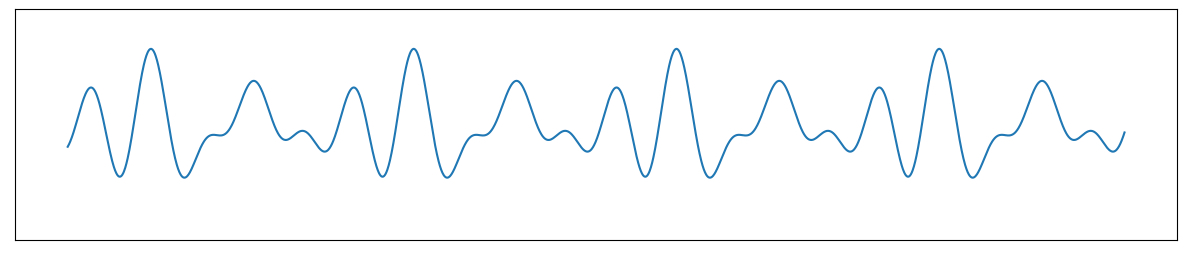
\includegraphics[scale=.35]{Mellin_00.jpg}
	$$
	\vskip -.4cm
	\caption{{\bf Real part of Mellin transform of $\pmb{f}$ and $\pmb{\omega}$ in Equations \eqref{equation: cslc f for Mellin 01} and \eqref{equation: norm un char for Mellin 00}.} [...]}
	\label{figure: Mellin 00}
	\end{figure}
	
\end{example}

\end{subsection}

\begin{subsection}{Using conductors to compute $\bold{GL}_1(\QQ_p)$-action on {\em p}-adic Mellin transforms}
\ {\color{red} [...]}

\begin{example}
{\bf Mellin transform of translation $\pmb{\rho_{a}\psi}$ of arbitrary character $\pmb{\psi:\ZZ^\times_p\lra\mathbb{S}^1}$.}
\normalfont
	$$
	\widetilde{{\rho_{a}\psi}}(s)
	\ \ =\ \ 
	\int_{\QQ^\times_{p}}
	\psi(a^{-1}x)\ \omega(x)\ |x|^{s}_{p}\ d^\times\!x,
	$$
Let $n$ be the conductor of $\omega$, and let $m$ be the conductor of $\psi$ (that is, before translating).

{\color{red} [...]}
\end{example}

\end{subsection}

\begin{subsection}{A gestural notation for $\bold{GL}_{1}(\QQ_p)$ signals.}
\ 
{\color{red} [...]}

\end{subsection}


\end{section}

\vskip 1cm

\begin{section}{Homogeneous polynomials and chords.}

\begin{subsection}{Sources}
	\begin{enumerate}[{\bf\ \ \ \ \ \ 1.}]
	\item
	[...]
	\end{enumerate}
\end{subsection}

\begin{subsection}{Decomposing complex numbers for better signal analysis}
Fix an element $z\in\CC$. Fixing a positive real {\em period} $P\in\RR_{>0}$ once and for all, we can decompose $z$ into its real and imaginary parts as
	\begin{equation}\label{complex decomp}
	z
	\ =\ 
	z(A,\theta)
	\ =\ 
	\text{log}(A)+i\tfrac{2\pi}{P}\theta,
	\end{equation}
for unique $0<A<\infty$ and $0\le \theta<P$. We refer to the positive real number $$\lambda:=\frac{1}{P}$$ as the {\em frequency} of $z(A,\theta)$. One reason for decomposing $z$ as in Equation \eqref{complex decomp} is that it gives the exponential of $z$ a form relevant to music. Indeed, from Equation \eqref{complex decomp} we get
	$$
	e^{z}
	\ =\ 
	A\ \!e^{i2\pi\lambda\theta},
	$$
with real and imaginary parts
	$$
	\text{Re}(e^{z})
	\ =\ 
	A\ \text{cos}(2\pi\lambda\theta)
	\ \ \ \ \ \ \ \ \ \text{and}\ \ \ \ \ \ \ \ \ 
	\text{Im}(e^{z})\ =\ A\ \text{sin}(2\pi\lambda\theta),
	$$
respectively. If we fix $A$ and let $\theta$ change linearly at the rate of $1$ unit per second, then both $\text{Re}(e^{z})$ and $\text{Im}(e^{z})$ describe a ``pure'' tone playing with amplitude $A$ at $\lambda\ \text{Hz}$. Here $A$ is measured in units of $A_0 \ e^{20\ \text{dB}}$, where $A_{0}$ is some fixed reference amplitude. The tone associated to $\text{Re}(e^{z})$ and the tone associated to $\text{Im}(e^{z})$ are out of phase by a quarter period $\frac{P}{4}$.

\end{subsection}

\begin{subsection}{Independent complex variables}
Suppose now that we choose two complex numbers $z_1,z_2\in\CC$, independently of one another, with corresponding exponentials
	\begin{equation}\label{same P}
	e^{z_1}
	=
	A_1\ e^{i2\pi\lambda\theta_1}
	\ \ \ \ \ \ \ \ \ \ \text{and}\ \ \ \ \ \ \ \ \ 
	e^{z_2}
	=
	A_2\ e^{i2\pi\lambda\theta_2}.
	\end{equation}
In Equation \eqref{same P}, we assume that we've fixed a single period $P$, hence a single frequency $\lambda$, that $z_1$ and $z_2$ share. However, we could just as well choose two different periods, $P_1$ and $P_2$ say, and thus two different frequencies $\lambda_1=\tfrac{1}{P_1}$ and $\lambda_2=\tfrac{1}{P_2}$, to get
	$$
	e^{z_1}
	=
	A_1\ e^{i\tfrac{2\pi}{P_1}\theta_1}
	=
	A_1\ e^{i2\pi\lambda_1\theta_1}
	\ \ \ \ \ \ \ \ \ \ \text{and}\ \ \ \ \ \ \ \ \ 
	e^{z_2}
	=
	A_2\ e^{i\tfrac{2\pi}{P_2}\theta_2}
	=
	A_2\ e^{i2\pi\lambda_2\theta_2},
	$$
where $\lambda_1=\tfrac{1}{P_1}$ and $\lambda_2=\tfrac{1}{P_2}$. 

Given a function $f(x,y)$ of two variables, we can evaluate $f$ at $x=e^{z_1}$ and $y=e^{z_2}$ to obtain the value $f(e^{z_1},e^{z_2})$. In the special case that $f(x,y)$ is a {\em Laurent monomial}, i.e., that
	$$
	f(x,y)=x^my^n,
	$$
for $m,n\in\ZZ$, we have
	$$
	f(e^{z_1}, e^{z_2})
	\ =\ 
	A_1A_2\ e^{i2\pi (m\lambda_1\theta_1+n\lambda_2\theta_2)}
	\ =\ 
	A_1A_2\ e^{i2\pi\big(\tfrac{m}{P_1}\theta_1+\tfrac{n}{P_2}\theta_2\big)}.
	$$
The real and imaginary parts of this are
	\begin{equation}\label{FM style 1}
	\text{Re}\ f(e^{z_1}, e^{z_2})
	\ =\ 
	A_1A_2\ \text{cos}\Big(2\pi\big(\tfrac{m}{P_1}\theta_1+\tfrac{m}{P_2}\theta_2\big)\Big)
	\end{equation}
	$$
	\ \ \ \ \ \ \text{and}\ \ \ \ \ \ 
	$$
	\begin{equation}\label{FM style 2}
	\text{Im}\ f(e^{z_1}, e^{z_2})
	\ =\ 
	A_1A_2\ \text{sin}\Big(2\pi\big(\tfrac{m}{P_1}\theta_1+\tfrac{m}{P_2}\theta_2\big)\Big)
	.
	\end{equation}
This is a situation ripe for techniques from frequency modulation. For instance, if we let $t$ denote our time variable, in units of seconds, and we define
	$$
	\theta_1(t)\ =\ t
	\ \ \ \ \ \ \ \ \ \text{and}\ \ \ \ \ \ \ \ \ 
	\theta_2(t)\ =\ \text{sin}(\omega\ \!t)\ \ \ \text{for some}\ \omega\in\RR_{>0},
	$$
then the formulas in Equations \eqref{FM style 1} and \eqref{FM style 2} become instances of \href{https://en.wikipedia.org/wiki/Frequency_modulation_synthesis}{{\em FM synthesis}}. We can also see that the formulas in Equations \eqref{FM style 1} and \eqref{FM style 2} give us a broad generalization of FM synthesis, in that we can use any pair of real-valued functions
	$$
	\theta_1(t)\ \ \ \ \ \ \text{and}\ \ \ \ \ \ \ \theta_2(t)
	$$
of $t$ that we like. In this way, a kind of generalized FM synthesis realizes one version of the notion of ``pitch movement in $2$ dimensions.'' See Figure \ref{figure: ring modulation 2 dimensions}.
%It is important to keep in mind that the linear independence between the $2$ dimensions here is happening in the logarithm. In other words, the linear independence is in the variable $z$, not in the value $e^{z}$.
	\begin{figure}[ht]
	$$
	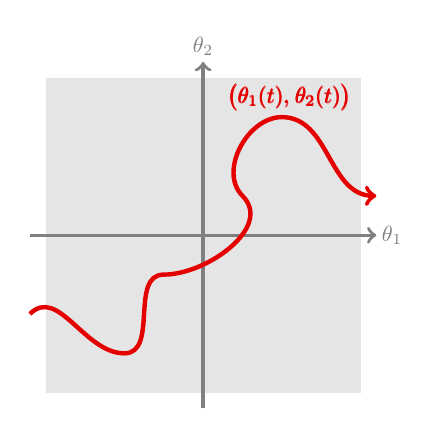
\begin{tikzpicture}
	\fill[black!10] (2,2) -- (-2,2) -- (-2, -2) -- (2, -2) -- cycle;
	\draw[black!50, very thick, ->] (-2.2,0) -- (2.2,0);
	\draw[black!50, very thick, ->] (0,-2.2) -- (0,2.2);
	\draw[red!90!black!100, ultra thick, ->] (-2.2,-1) to [out=45, in=180] (-1,-1.5) to [out=0, in=180] (-.5,-.5) to [out=0, in=-45] (.5,.5) to [out=135, in=180] (1, 1.5) to [out=0, in=180] (2.2,.5);
	\node[black!50] at (2.4, 0) {\scalebox{.8}{$\theta_1$}};
	\node[black!50] at (0, 2.4) {\scalebox{.8}{$\theta_2$}};	
	\node[red!90!black!100] at (1.1, 1.75) {\scalebox{.8}{$\pmb{\big(\theta_1(t),\ \!\theta_2(t)\big)}$}};
	\end{tikzpicture}
	$$
	\caption{General FM-synthesis from curves in the real plane.}
	\label{figure: ring modulation 2 dimensions}
	\end{figure}

%This begins to move into the realm of harmony. We pause our development of harmony here, and pick it back up in {\color{red} \S[...]}

\begin{example}
\normalfont
{\bf Ring modulation as a special case.}
Let us briefly remark here that, although it is not usually presented in this way, {\em ring modulation} in signal processing arises when we evaluate the real and imaginary parts of the monomial $xy$ at $x=e^{z_1}$ and $y=e^{z_2}$. In this way, ring modulation becomes a special case of the above discussion.
\end{example}

\begin{example}
\normalfont
{\bf Logarithmic representations.}
Consider the case of a single complex-valued function $z(t)=i2\pi\lambda t$ of the real variable $t$. How might we transform such a function. One obvious way is to consider all {\em $\RR$-affine transformations} of $t$, that is, all transformations that can be described by an $\RR$-linear polynomial:
	$$
	t
	\ \longmapsto\ 
	a+bt.
	$$
The group of all such transformations is denoted $\text{Aff}(\RR)$. It admits a normal decomposition
	$$
	0
	\longrightarrow
	\RR
	\longrightarrow
	\text{Aff}(\RR)
	\longrightarrow
	\RR^\times
	\longrightarrow
	1
	$$
that gives this group a semidirect product decomposition
	$$
	\text{Aff}(\RR)\ \cong\ \RR\rtimes\RR^\times.
	$$
We can effectively ``mod out'' the {\em translation} action by the normal subgroup $\RR\lhd\text{Aff}(\RR)$ by focus on the action of the non-normal, multiplicative subgroup $\RR^{\times}\subset\text{Aff}(\RR)$.

If we work with $e^{z}=e^{i2\pi\lambda t}$, the translation action $t\mapsto a+t$ by the normal subgroup $\mathbb{R}\rtimes\text{Aff}(\RR)$ amounts to phase shifting, as it takes
	$$
	e^{i2\pi\lambda t}
	\ \longmapsto\ 
	e^{i(2\pi\lambda t+\phi)},
	\ \ \ \text{where}\ 
	\phi=2\pi\lambda a.
	$$
If we take a musical perspective that ignores the effects of phase shifting, then we can focus on the action of the non-normal multiplicative subgroup $\RR^\times\subset\text{Aff}(\RR)$. It is common to use logarithmic coordinates for this group by writing $b=e^{s}$. We obtain transformations of the form
	$$
	e^{i2\pi\lambda t}
	\ \longmapsto\ 
	e^{i2\pi\lambda e^s t}.
	$$
Writing $\lambda=e^{s_0}$, this becomes
	$$
	e^{i2\pi e^{s_0} t}
	\ \longmapsto\ 
	e^{i2\pi e^{s_0+s} t}.
	$$
The charged particle dynamics in {\em Voice Leader\ \textemdash\ DISPL.} take place in something like the Lie algebra of the multiplicative group $\RR^\times$ that acts on the frequency specturm. Ignoring the negative component of this Lie algebra amounts to the assertion that we do not consider backward movement through time in musical contexts.

This leads us to the following questions for the case of $2$ independent variables $z_1$ and $z_2$.
\end{example}

\begin{question}
\normalfont
What is the right ``space'' to do dynamics in when there are two variables?... (frequency or log-frequency). 

There are going to be competing pictures, throughout these notes, for what level ``space'' should be taken at...
\end{question}

\begin{question}
\normalfont
What is the Lie bracket on the tangent space $T_{(\bold{q},\bold{p})}M$ of phase space $M$ at a state $(\bold{q},\bold{p})$?

\vskip .2cm

{\em Answer.} {\color{red} [Poisson algebra structure on the space of functions. The Lie algebra structure on the tangent space itself is known as the symplectic Lie algebra or the Lie algebra of Hamiltonian vector fields...]}

\vskip .2cm

{\em Relevance of the question to representations of algebraic groups.} {\color{red}\bf [...]}
\end{question}

\end{subsection}

\vskip .2cm

\begin{subsection}{Ring modulation versus products in representation theory}
	In representation theory, products arise from tensor constructions like tensor powers $V^{\otimes n}$, symmetric powers $\text{Sym}^{n}V$, and exterior powers $\Lambda^{n}V$ of representations $V$. The basic example of an element in one of these representations is the symmetric product $xy$ of two complex variables $x$ and $y$. If we're thinking in terms of irreducible representations, then it is natural to take 
	\begin{equation}\label{equation: variable assignment for product}
	x\ =\ e^{i2\pi\lambda t}
	\ \ \ \ \ \ \ \ \ \text{and}\ \ \ \ \ \ \ \ \ 
	y=e^{i2\pi\mu t}.
	\end{equation}
In this case, we have
	$$
	xy\ =\ e^{i2\pi(\lambda+\mu)\ \!t}.
	$$
Notice that here, products correspond to addition of frequencies.

	Ring modulation, on the other hand, corresponds to the product
	$$
	\text{Re}(x)\cdot\text{Re}(y).
	$$
If we let $x$ and $y$ take the values in Equation \ref{equation: variable assignment for product}, then this ring modulation product
	$$
	\text{sin}(2\pi\lambda t)\cdot\text{sin}(2\pi\mu t).
	$$
[...]
	\begin{equation}\label{equation: first expansion}
	\begin{array}{rcl}
	e^{i2\pi(\lambda+\mu)\ \!t}
	& \!\!=\!\!
	& \text{cos}\big(2\pi(\lambda+\mu)\ \!t\big)+i\ \text{sin}\big(2\pi(\lambda+\mu)\ \!t\big)
	\end{array}
	\end{equation}
[...]
	\begin{equation}\label{equation: second expansion}
	\begin{array}{rcl}
	e^{i2\pi\lambda t}\cdot e^{i2\pi\mu t}
	& \!\!=\!\!
	& \big(\text{cos}(2\pi\lambda t)+i\ \text{sin}(2\pi\lambda t)\big)
	\cdot
	\big(\text{cos}(2\pi\mu t)+i\ \text{sin}(2\pi\mu t)\big)
	\\[6pt]
	& \!\!=\!\!
	& \ \ \ \ \ \ \ \!\big(
	\text{cos}(2\pi\lambda t)\ \!\text{cos}(2\pi\mu t)
	-
	\text{sin}(2\pi\lambda t)\ \!\text{sin}(2\pi\mu t)
	\big)
	\\[6pt]
	&
	& 
	+\ i\ 
	\big(\text{cos}(2\pi\lambda t)\text{sin}(2\pi\mu t)+\text{sin}(2\pi\lambda t)\text{cos}(2\pi\mu t)\big)
	\end{array}
	\end{equation}
Identifying Equations \eqref{equation: first expansion} and \eqref{equation: second expansion}, we have
	\begin{equation}\label{equation: fragment A}
	\text{sin}(2\pi\lambda t)\cdot\text{sin}(2\pi\mu t)
	\ =\ 
	\text{cos}(2\pi\lambda t)\ \!\text{cos}(2\pi\mu t)
	-
	\text{cos}\big(2\pi(\lambda+\mu)\ \!t\big).
	\end{equation}
[...]
	\begin{equation}\label{equation: third expansion}
	\begin{array}{rcl}
	e^{i2\pi(\lambda-\mu)\ \!t}
	& \!\!=\!\!
	& \text{cos}\big(2\pi(\lambda-\mu)\ \!t\big)+i\ \text{sin}\big(2\pi(\lambda-\mu)\ \!t\big)
	\end{array}
	\end{equation}
[...]	\begin{equation}\label{equation: fourth expansion}
	\begin{array}{rcl}
	e^{i2\pi\lambda t}\cdot e^{-i2\pi\mu t}
	& \!\!=\!\!
	& \big(\text{sin}(2\pi\lambda t)+i\ \text{cos}(2\pi\lambda t)\big)
	\cdot
	\big(-\text{sin}(2\pi\mu t)+i\ \text{cos}(2\pi\mu t)\big)
	\\[6pt]
	& \!\!=\!\!
	& \ \ \ \ \ \ \ \!\big(
	-\text{sin}(2\pi\lambda t)\ \!\text{sin}(2\pi\mu t)
	-
	\text{cos}(2\pi\lambda t)\ \!\text{cos}(2\pi\mu t)
	\big)
	\\[6pt]
	&
	& 
	+\ i\ 
	\big(\text{sin}(2\pi\lambda t)\text{cos}(2\pi\mu t)-\text{cos}(2\pi\lambda t)\text{sin}(2\pi\mu t)\big)
	\end{array}
	\end{equation}
Identifying Equations \eqref{equation: third expansion} and \eqref{equation: fourth expansion}, we have
	\begin{equation}\label{equation: fragment B}
	\text{cos}(2\pi\lambda t)\cdot\text{cos}(2\pi\mu t)
	\ =\ 
	-\text{sin}(2\pi\lambda t)\ \!\text{sin}(2\pi\mu t)
	-
	\text{cos}\big(2\pi(\lambda-\mu)\ \!t\big).
	\end{equation}
Putting Equations \eqref{equation: fragment A} and \eqref{equation: fragment B} together, we arrive at the identity
	$$
	2\ \text{sin}(2\pi\lambda t)\ \!\text{sin}(2\pi\mu t)
	\ =\ 
	\text{cos}\big(2\pi(\lambda+\mu)\ \!t\big)+\text{cos}\big(2\pi(\lambda-\mu)\ \!t\big),
	$$
more commonly written
	\begin{equation}\label{equation: trig identity}
	\text{sin}(2\pi\lambda t)\cdot\text{sin}(2\pi\mu t)
	\ =\ 
	\frac{1}{2}\text{cos}\big(2\pi(\lambda+\mu)\ \!t\big)+\frac{1}{2}\text{cos}\big(2\pi(\lambda-\mu)\ \!t\big)
	\end{equation}

	The point of all of this is that we have competing interpretations of signal multiplication coming from the inequality
	$$
	\text{Re}(xy)\ \neq\ \text{Re}(x)\cdot\text{Re}(y)
	$$
for complex variables $x$ and $y$.
	
\begin{question}
{\bf A purely Galois version of the identity in Equation \eqref{equation: trig identity}?}
\normalfont
We can re-interpret the factor $e^{-i2\pi\mu t}$ in Equation \eqref{equation: fourth expansion} as the Galois conjugate
	$$
	e^{-i2\pi\mu t}=\sigma(e^{i2\pi\mu t}),
	$$
where $\sigma$ denotes the unique non-trivial automorphism in $\text{Gal}(\CC/\RR)$. In this way, the identity in Equation \eqref{equation: trig identity} can be written in the non-trigonometric form
	\begin{equation}\label{equation: non-trig form}
	\text{Re}(x)\text{Re}(y)
	\ =\ 
	\frac{1}{2}\text{Re}(xy)+\frac{1}{2}\text{Re}\big(x\cdot\sigma(y)\big).
	\end{equation}
We can think of the $\RR$-linear map $\text{Re}:\CC\longrightarrow\RR$ as a projection operation with respect to the $\RR$-linear basis $\{1,i\}$ in $\CC$, where $i$ is a root of the irreducible quadratic polynomial $x^2+1\in\RR[x]$. If we let $\omega$ be the root of some other irreducible quadratic polynomial $x^2+ax+b\in\RR[x]$, we get a new $\RR$-linear basis $\{1,\omega\}$ for $\CC$, and thus a {\em new} projection
	$$
	\text{pr}_{\omega}:\CC\longrightarrow\RR.
	$$
Is it the case that this new projection satisfies the naive analogue of Equation \eqref{equation: non-trig form}, namely
	$$
	\text{pr}_{\omega}(x)\text{pr}_{\omega}(y)
	\ =\ 
	\frac{1}{2}\text{pr}_{\omega}(xy)+\frac{1}{2}\text{pr}_{\omega}\big(x\cdot\sigma(y)\big)?
	$$
My first guess is that this can't be correct, and that it requires some modification coming from the polynomial $x^2+ax+b$.

	A further generalization might be some formula for any ``norm-type'' product
	$$
	\prod_{j,g\in\text{enum}\big(\text{Gal}(E/F)\big)}
	\!\!\!\!\!\!\!\!\!\!\!g(x_{j}).
	$$
My initial guess would be something of the form
	$$
	\prod_{j,g\in\text{enum}\big(\text{Gal}(E/F)\big)}
	\!\!\!\!\!\!\!\!\!\!\!g(x_{j})
	\ \ \ =\ \ \ 
	\frac{1}{\#\text{Gal}(E/F)}
	\sum_{g\in\text{Gal}(E/F)}\!\!\!\!\!\big(?\big)
	$$
Probably the right place to look for the answer is some general ``norm-to-trace'' formula in class field theory.
\end{question}
	
\end{subsection}

\vskip .2cm

\begin{subsection}{Homogenous linear combinations of independent complex variables}
If $x$ and $y$ are independent complex variables, then a $\CC$-linear combination of monomials in $x$ and $y$, say
	\begin{equation}\label{homogeneous linear comb 1}
	a_{1}x^{m_1}y^{n_1}
	+
	a_{2}x^{m_2}y^{n_2}
	+
	\cdots
	+
	a_{\ell}x^{m_\ell}y^{n_\ell},
	\ \ \ a_1,a_2,\dots,a_\ell\in\CC
	\end{equation}
is {\em homogeneous of degree $d$} if $m_i+n_i=d$ for all $1\le i\le \ell$, in other words, if all monomials $x^my^n$ in the linear combination have the same {\em total degree} $m+n$, equal to $d$. When the linear combination in Equation \eqref{homogeneous linear comb 1} is homogeneous of degree $d$, we refer to it as a {\em homogeneous polynomial of degree $d$} in the variables $x$ and $y$ over $\CC$.

Notice that, from a musical perspective, a homogeneous linear combination in Equation \eqref{homogeneous linear comb 1} combines two distinct ideas in a way that isn't possible with a single variable. It packages multiple instances of ring modulation into a single chord-like structure. Indeed, 

The general homogeneous polynomial of degree $d$ in $x$ and $y$ can be written
	$$
	f(x,y)
	\ =\ 
	a_{0}x^d+a_1x^{d-1}y+a_2x^{d-2}y^2+\cdots+a_{d-1}xy^{d-1}+a_{d}y^d,
	$$
with coefficients $a_0,a_1,\dots,a_d\in\CC$. We can write this more succinctly as
	$$
	f(x,y)
	\ =\ 
	\sum_{n=0}^{d}a_nx^{d-n}y^n.
	$$
Evaluating this polynomial at $x=e^{z_1}$ and $y=e^{z_2}$, we obtain
	\begin{equation}\label{equation: homogeneous eval at e^z}
	f(e^{z_1},e^{z_2})
	\ =\ 
	\sum_{n=0}^{d}a_{n}A_{1}^{d-n}A_{2}^{n}e^{i2\pi\big(\tfrac{d-n}{P_1}\theta_1+\tfrac{n}{P_2}\theta_2\big)}.
	\end{equation}
To get a slightly clearer picture of this, let us assume that $a_i=1$ for all $0\le i\le d$ {\color{red} [change $i$ to different letter...]} and that $A_1=A_2=1$. Then the right-hand side of Equation \eqref{equation: homogeneous eval at e^z} becomes
	\begin{equation}\label{equation: all amplitudes =1}
	\sum_{n=0}^{d}e^{i2\pi\big(\tfrac{d-n}{P_1}\theta_1+\tfrac{n}{P_2}\theta_2\big)}.
	\end{equation}
We play with this expression a bit more in Example \ref{example: relationship to standard chords} below.

\begin{example}\label{example: relationship to standard chords}
\normalfont
{\color{red} [...]}

{\bf Special case: $\pmb{\theta_1=\theta_2}$ and $\pmb{P_1=P_2}$.}
{\color{red} [...]}
	Equation \eqref{equation: all amplitudes =1} becomes
	$$
	(d+1)e^{i2\pi\tfrac{d}{P}\theta}
	\ =\ 
	(d+1)e^{i2\pi d\lambda\theta}
	$$

{\bf Special case: $\pmb{\theta_1=0}$.}
{\color{red} [...]}
	Equation \eqref{equation: all amplitudes =1} becomes
	$$
	\sum_{n=0}^{d}e^{i2\pi\tfrac{n}{P}\theta}
	\ =\ 
	1
	+
	e^{i2\pi\tfrac{1}{P}\theta}
	+
	e^{i2\pi\tfrac{2}{P}\theta}
	+
	\dots
	+
	e^{i2\pi\tfrac{d}{P}\theta},
	$$
or in terms of frequency,
	$$
	f(1,e^{i2\pi\lambda\theta})
	\ =\ 
	1
	+
	e^{i2\pi \lambda\theta}
	+
	e^{i2\pi 2\lambda\theta}
	+
	\dots
	+
	e^{i2\pi d \lambda\theta}.
	$$
Ignoring the constant term ``$1$,'' this is just an equi-voiced\footnote{\ We say that a chord is {\em equi-voiced} if the notes of a chord are equally loud. I don't know if this is standard terminology.} overtone chord with root at $\lambda\ \text{Hz}$, and including overtones $1$ through $d$.

If we let $A_1=1$ and $A_2=\varepsilon$, where $0<\varepsilon <1$, then this becomes
	$$
	f(1,\varepsilon e^{i2\pi\lambda\theta})
	\ =\ 
	1
	+
	\varepsilon e^{i2\pi \lambda\theta}
	+
	\varepsilon^2 e^{i2\pi 2\lambda\theta}
	+
	\dots
	+
	\varepsilon^d e^{i2\pi d \lambda\theta}.
	$$
This is the same overtone chord, but with voicing that falls of like a geometric series as we move up the overtone scale.
\end{example}

\begin{question}
\normalfont
{\color{red} [Voicing and orchestration questions...]}
\end{question}


\begin{remark}
\normalfont
{\color{red} [Model movement of several $(\theta_1,\ \theta_2)$-pairs on particle dynamics in $2$-dimensional space. This provides an FM version of the particle dynamics experiment from {\em Voice Leader\ \textemdash\ DISPL.}...]}
\end{remark}
[...]
\end{subsection}

\begin{subsection}{A gestural notation.}
\ 
{\color{red} [...]}

\end{subsection}

\end{section}

\vskip 1cm

\begin{section}{Representations of the special linear group $\bold{SL}_{2}(\CC)$.}

\begin{subsection}{Sources}
	\begin{enumerate}[{\bf\ \ \ \ \ \ 1.}]
	\item
	\cite{FH}
	\item
	\cite{Proc}
	\item
	\cite{Knapp86}
	\item
	\cite{Knapp02}
	\end{enumerate}
\end{subsection}

\begin{subsection}{The Cartan-Weyl basis.} The $3$-dimensional Lie algebra
	$$
	\mathfrak{sl}_2(\CC)
	\ =\ 
	\left\{
	\left(\!\begin{array}{cc}a & b \\ c & \!\!-a\end{array}\!\right)\in\text{Mat}_{2\times2}(\CC)
	\right\}
	$$
admits a standard basis, sometimes called the {\em Cartan-Weyl basis}, given by
	$$
	E:=\left(\!\begin{array}{cc}0 & 1 \\ 0 & 0\end{array}\!\right),
	\ \ \ \ \ \ 
	H:=\left(\!\begin{array}{cc}1 & 0 \\ 0 & \!\!-1\end{array}\!\right),
	\ \ \ \ \ \ 
	\text{and}
	\ \ \ \ \ \ 
	F:=\left(\!\begin{array}{cc} 0 & 0 \\ 1 & 0\end{array}\!\right).
	$$
The $1$-parameter subgroups gotten by exponentiation of these basis vectors have general element
	$$
	e^{zE}
	\ =\ 
	\text{I}+zE+\frac{z^2}{2}{\color{red} \cancelto{0}{{\color{black} E^2}}}+\frac{z^3}{3!}{\color{red} \cancelto{0}{{\color{black} E^3}}}+\cdots
	\ =\ 
	\left(\!\begin{array}{cc} 1 & z \\ 0 & 1\end{array}\!\right),
	$$
	$$
	e^{zF}
	\ =\ 
	\text{I}+zF+\frac{z^2}{2}{\color{red} \cancelto{0}{{\color{black} F^2}}}+\frac{z^3}{3!}{\color{red} \cancelto{0}{{\color{black} F^3}}}+\cdots
	\ =\ 
	\left(\!\begin{array}{cc} 1 & 0 \\ z & 1\end{array}\!\right),
	$$
and
	$$
	\begin{array}{rclcl}
	e^{zH}
	& \!\!=\!\! &
	I+zH+\frac{z^2}{2}H^2+\frac{z^3}{3!}H^3+\cdots
	\\[20pt]
	& \!\!=\!\! &
	\left(\ \!\begin{array}{cc} 1+z+\tfrac{z^2}{2}+\tfrac{z^3}{3!}+\cdots & 0 \\[7pt] 0 & 1-z+\tfrac{z^2}{2}-\tfrac{z^3}{3!}+\cdots\end{array}\!\ \right)
	& \!\!=\!\! &
	\left(\!\begin{array}{cc} e^z & 0 \\ 0 & e^{-z}\end{array}\!\right),
	\end{array}
	$$
respectively. One recurring theme in these notes is the question ``should we work in the space where our variable is $z$, or in the space where are variable is $q=e^{z}$. Note, though, that this distinction gets confused in $\bold{SL}_{2}(\CC)$, since the complex parameter $z$ acts by multiplication directly in the $1$-parameter subgroups $$\{e^{zE}:z\in\CC\}\ \ \text{and}\ \ \{e^{zF}:z\in\CC\}\subset\bold{SL}_{2}(\CC),$$ but acts through multiplication by in the $1$-parameter subgroup $$\{e^{zH}:z\in\CC\}\subset\bold{SL}_{2}(\CC).$$

Every element $\left(\begin{smallmatrix} a & b \\ c & d\end{smallmatrix}\right)\in\bold{SL}_{2}(\CC)$ admits a factorization
	$$
	\left(\!\begin{array}{cc}a & b \\ c & d\end{array}\!\right)
	\ =\ 
	e^{u E}e^{v H}e^{w F}
	\ =\ 
	\left(\!\begin{array}{cc}1 & w \\ 0 & 1\end{array}\!\right)
	\left(\!\begin{array}{cc}e^{v} & 0 \\ 0 & e^{-v}\end{array}\!\right)
	\left(\!\begin{array}{cc}1 & 0 \\ u & 1\end{array}\!\right)
	$$
for some $u,v,w\in\CC$ {\color{red} [Not true. A certain conjugation is needed to get matrices $\left(\begin{smallmatrix} 0 & b \\ \!\!-\tfrac{1}{b} & 0\end{smallmatrix}\right)$... What is the correct statement here. Some kind of decomposition theorem for the Lie group?...Bruhat decomposition?...]}. To compute $u,v,w$, observe that the matrix product on the right is equal to
	$$
%	\left(\!\begin{array}{cc}1 & w \\ 0 & 1\end{array}\!\right)
%	\left(\!\begin{array}{cc}e^v & 0 \\ ue^{-v} & e^{-v}\end{array}\!\right)
%	\ =\ 
	\left(\!\begin{array}{cc}e^v+uwe^{-v} & we^{-v} \\ ue^{-v} & e^{-v}\end{array}\!\right),
	$$
hence
	$$
	d=e^{-v},
	\ \ \ \ \ \ 
	w=b/d,
	\ \ \ \ \ \ 
	u=c/d
	$$
{\color{red} [...confusing myself... need to come back to this...]} The thing that's confusing me is how $\left(\begin{smallmatrix} 0 & b \\ \!\!-\tfrac{1}{b} & 0\end{smallmatrix}\right)$ appears. Maybe the 1-parameter subgroups at the identity $I=\left(\begin{smallmatrix} 1 & 0 \\ 0 & 1\end{smallmatrix}\right)\in\bold{SL}_{2}(\CC)$ doesn't reach any of the cell
	\begin{equation}\label{stratum 1}
	S:=\left\{\left(\begin{smallmatrix} 0 & b \\ \!\!-\tfrac{1}{b} & 0\end{smallmatrix}\right):b\in\CC^\times\right\}
	\ \subset\ 
	\bold{SL}_{2}(\CC).
	\end{equation}
What is the product of two elements of this cell like?
	$$
	\left(\begin{matrix} 0 & b \\ \!\!-\tfrac{1}{b} & 0\end{matrix}\right)
	\left(\begin{matrix} 0 & -\tfrac{1}{c} \\ c & 0\!\!\end{matrix}\right)
	\ =\ \left(\begin{matrix} bc & 0 \\ 0 & \tfrac{1}{bc}\end{matrix}\right)
	\ \in\ \{e^{zH}:z\in\CC\}.
	$$
In other words, the square of the stratum defined in Equation \eqref{stratum 1} is the $1$-parameter subgroup generated by the exponentiation of the basis field $H\in\mathfrak{sl}_{2}(\CC)$.



{\color{red} [Factorizations coming from other permutations of these $3$ factors...]}

{\color{red} [...]}
\end{subsection}

\begin{subsection}{Action of $\bold{SL}_{2}(\CC)$ on $\CC[x,y]$}
We let $\bold{SL}_{2}(\CC)$ act on $\CC[x,y]$ through its inverse action on the argument $(x,y)$ of each function $f(x,y)\in\CC[x,y]$. Thus the matrix $\left(\begin{smallmatrix}a & b\\ c & d\end{smallmatrix}\right)\in\bold{SL}_{2}(\CC)$ acts on each $f(x,y)\in\CC[x,y]$ via the action of its inverse $\left(\begin{smallmatrix}d & -b\ \\ -c\  & a\end{smallmatrix}\right)$
\end{subsection}

\begin{subsection}{Irreducible representations of $\text{SL}_2(\CC)$ in $\CC[x,y]$}
[...]
\end{subsection}

\begin{subsection}{The irreducible $2$-dimensional representation of $\text{SL}_2(\CC)$}
[...]
\end{subsection}

\begin{subsection}{The irreducible $3$-dimensional representation of $\text{SL}_2(\CC)$}
[...]
\end{subsection}

\begin{subsection}{``Harmonic movement'' for $\text{SL}_2(\CC)$}

\begin{question}\label{question: what is harmonic movement}
\normalfont
What sort of movement through the category $\bold{Rep}\big(\bold{SL}_{2}(\CC)\big)$ is the ``correct'' generalization of the movement through $\bold{Rep}\big(\mathbb{S}^{1}\big)$ that corresponds to $\ZZ$-multiplicative movement through the terms of a Fourier series?

\vskip .3cm

\noindent
{\em Temporary answers.} As we pointed out on \S\ref{subsection: Competing interpretations of harmonic and tonal movement}, there are competing interpretations of standard tonal and harmonic and tonal movement within $\bold{Rep}(\mathbb{S}^1)$ or $\bold{Rep}\big(\bold{GL}_{1}(\CC)\big)$. Because meany There are many reasonable candidates:
	\begin{enumerate}[{\em\ \ \ \ \ \ {Answer \ref{question: what is harmonic movement}.}1.}]
	\item
	Inductive/restrictive functorial movement along homomorphisms $G\longrightarrow\bold{SL}_{2}(\CC)$ and/or $\bold{SL}_{2}(\CC)\longrightarrow G$;
	\item
	Movement along functors $\text{Hom}(V_{n},-)$;
	\item
	Movement along functors $T^{n}=(-)^{\otimes n}$;
	\item
	Movement along functors $\text{Sym}^{n}$.
	\end{enumerate}
There are also candidates for new types of harmonic movement:
	\begin{enumerate}[{\em\ \ \ \ \ \ {New possibility \ref{question: what is harmonic movement}.}5.}]
	\item
	Movement along functors $\Lambda^{n}$.
	\end{enumerate}
{\color{red} [Explain issue of plethysm/fusion rules...]}
\end{question}

[...]
\end{subsection}

\begin{subsection}{Plethysm}
[...]
\end{subsection}

\begin{subsection}{A gestural notation.}
\ 
{\color{red} [...]}

\end{subsection}

\end{section}

\vskip 1cm

\begin{section}{Hamiltonian optics and representations of the symplectic group $\text{Sp}_{2n}(\CC)$}

\begin{subsection}{Sources}
	\begin{enumerate}[{\bf\ \ \ \ \ \ 1.}]
	\item
	\cite{GS}
	\end{enumerate}
\end{subsection}
[...]
\end{section}

\vskip 1cm

\begin{section}{Homogeneous spaces}

\begin{subsection}{Sources}
	\begin{enumerate}[{\bf\ \ \ \ \ \ 1.}]
	\item
	\cite{Serre}
	\item
	\cite{Tim}
	\item
	\cite{Schmitt}
	\end{enumerate}
\end{subsection}

\end{section}

%$$
%10,668,000
%\ =\ 
%\left(\!\!
%\begin{array}{c}
%128\\
%4
%\end{array}
%\!\!\right)
%$$
%
%$$
%\mathbb{E}[f]
%\ =\ 
%\int_{S}f(s)ds
%$$
%
%$$
%\underset{
%{\smaller\smaller\smaller\smaller\smaller
%\begin{array}{c}
%\text{paths $\gamma$ in $S$}
%\\
%\text{starting at $s$}
%\end{array}
%}
%}{\text{argmax}}
%\ G(\gamma)
%$$
%
%$$
%\mathbb{E}_\pi[G|s]
%\ =\ 
%\int_{\!\!\mathscr{P}\!(S,s)}\!\!\!\!G(\gamma)\ d\pi
%$$
%
%$$
%\mathbb{E}_{\pi}[G|s]
%\ =\!\!
%\underset{
%{\smaller\smaller\smaller\smaller
%\begin{array}{c}
%\text{actions}
%\\
%\alpha\ \text{at}\ s
%\end{array}
%}
%}{\sum}
%\!\!\!\!
%\Big(
%\Delta_{\alpha}G
%+
%\mathbb{E}\big[G\big|\alpha(s)\big]
%\Big)
%\ 
%p_{\pi}(\alpha|s)
%$$
%
%$$
%\Big(
%\Delta_{\beta}G
%+
%\mathbb{E}\big[G\big|\beta\!\circ\!\alpha(s)\big]
%\Big)\
%$$
%
%$$
%\mathbb{E}_{\pi}[G|\alpha,s]
%\ =\ 
%\Delta_{\alpha}G
%+
%\mathbb{E}\big[G\big|\alpha(s)\big]
%$$
%
%$$
%\mathbb{E}_{\pi}[G|\alpha,s]
%\ =\ 
%\Delta_{\alpha}G
%\ +\!\!\!\!\!\!
%\underset{
%{\smaller\smaller\smaller\smaller
%\begin{array}{c}
%\text{actions}
%\\
%\beta\ \text{at}\ \alpha(s)
%\end{array}
%}
%}{\sum}
%\!\!\!\!
%\mathbb{E}\big[G\big|\beta,\alpha(s)\big]
%\cdot
%p_{\pi\!}\big(\beta\big|\alpha(s)\big)
%$$
%
%$$
%\mathbb{E}_{\pi}[G|\alpha,s]
%\ =\ 
%\Delta_{\alpha}G
%\ +\ 
%\mathbb{E}\big[G\big|\beta_{\text{{\smaller\smaller\smaller\smaller\smaller best}}},\alpha(s)\big]
%$$
%
%$$
%\mathbb{E}[G|\alpha_i,s_i]
%\ =\ 
%R_{\alpha_i}+R_{\alpha_{i+1}}+R_{\alpha_{i+2}}+\cdots+R_{\alpha_n}
%$$
%
%$$
%\begin{array}{rcl}
%\mathscr{L}(\alpha, s)
%&
%\!\!:=\!\!
%& 
%\mathbb{E}[G|\alpha,s]\cdot\text{log}\Big(\frac{1}{\mathscr{Q}(\alpha, s)}\Big)
%\\[12pt]
%&
%\!\!=\!\!
%&
%\Big(\underset{\beta\ge\alpha}{\scalebox{1.2}{$\sum$}}R_{\beta}\Big)
%\cdot
%\text{log}\Big(\frac{1}{\mathscr{Q}(\alpha, s)}\Big)
%\end{array}
%$$








\vskip .75cm

\bibliographystyle{alpha}
\bibliography{SL_2C}

\end{document}
